\documentclass[a4paper]{article}    % define document layout
%\documentclass[draft]{article}     % use draft option in packages
%-----------------------------
% preamble
%-----------------------------
\usepackage[sumlimits,]{amsmath}    % math equations and formulas
\usepackage[utf8]{inputenc}         % use UTF-8 encoding
\usepackage[english]{babel}         % use English language
\usepackage{graphicx}              % insert images
%\usepackage[draft]{graphicx}        % do not render figures
\usepackage{subcaption}             % multiple images in one figure
\usepackage{hyperref}               % hyperlinks
\usepackage{float}                  % floating objects (figures, tables)
\usepackage{geometry}               % page size and margins
\geometry{a4paper, margin=1in}      % margins
\usepackage{ragged2e}               % text alignment
\usepackage[table]{xcolor}          % change cell color in tables
%\usepackage{multirow}               % merge rows in table

\graphicspath{                      % path for figures
    {../figures/} 
    {../figures/alpha/} 
    {../figures/cm/} 
    {../figures/heatmap/} 
    {../figures/misclassified/} 
}

%-----------------------------
% body
%-----------------------------
\begin{document}

\begin{figure}
    \centering
    % UNICAMP logo
    \begin{subfigure}{0.45\textwidth}
        \centering
        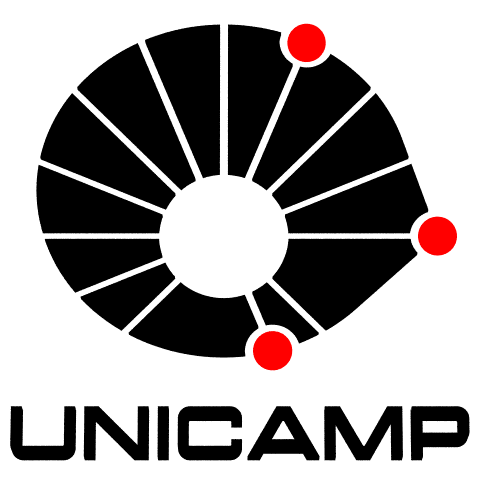
\includegraphics[width=1.5cm]{unicamp}
%        \label{fig:unicamp}
    \end{subfigure}
    \hfill
    % FEEC logo
    \begin{subfigure}{0.45\textwidth}
        \centering
        
\includegraphics[width=1.5cm]{feec}
%        \label{fig:feec}
    \end{subfigure}
\end{figure}

\title{EFC1 - Exercise 1}
\author{Rafael Claro Ito (R.A.: 118430)}
%R.A.: 118430
%ito.rafael@gmail.com
\date{April 2020}
\maketitle
\newpage

%=================================================
\section{Source files}
%=================================================

\paragraph{The Jupyter notebook with the code used to generate the plots and results presented in this report, all figures showed here and even the \LaTeX \space source code used to generate this PDF can be found at the following GitHub repository:}

\begin{center}
    {\url{https://github.com/ito-rafael/IA353A-NeuralNetworks-1s2020}}
\end{center}

%=================================================
\section{Regularization coefficient (Ridge Regression)}
%=================================================

%=================================================
\subsection{Results summary}
%=================================================

\begin{table}[H]
    \begin{center}
        \begin{tabular}{r|c|c|} 
            \cline{2-3}
            & \multicolumn{2}{|c|}{\cellcolor[gray]{0.8}{$\lambda$ optimum}} \\
            \cline{2-3}
            & \cellcolor[gray]{0.8}{MSE} & \cellcolor[gray]{0.8}{Accuracy} \\
            \cline{1-3}
            \multicolumn{1}{|r|}{\cellcolor[gray]{0.8}{coarse search}} & 64   & 1024   \\
            \cline{1-3}
            \multicolumn{1}{|r|}{\cellcolor[gray]{0.8}{fine search}}   & 51.5 & 1091.8 \\
            \cline{1-3}
        \end{tabular}
    \end{center}
    \caption{Values of regularization coefficient found in coarse and fine searches}
    \label{tab:alpha_results}
\end{table}

%=================================================
\subsection{Coarse search}
%=================================================

\paragraph{While performing the coarse search for the best regularization coefficient, 3 more values of lambda were added. This was done in order to see the falling of the accuracy curve, since the last suggested value, $2^{10}$, had the best accuracy. The final values of lambda tested were:}

\begin{center}
    alpha\_interval = $[2^{-10}, 2^{-8}, 2^{-6}, 2^{-4}, 2^{-2}, 2^{0}, 2^{2}, 2^{4}, 2^{6}, 2^{8}, 2^{10}, \boldsymbol{2^{11}, 2^{12}, 2^{13}}]$
\end{center}

\begin{figure}[H]
    \centering
    % digit 0
    \begin{subfigure}{0.48\textwidth}
        \centering
        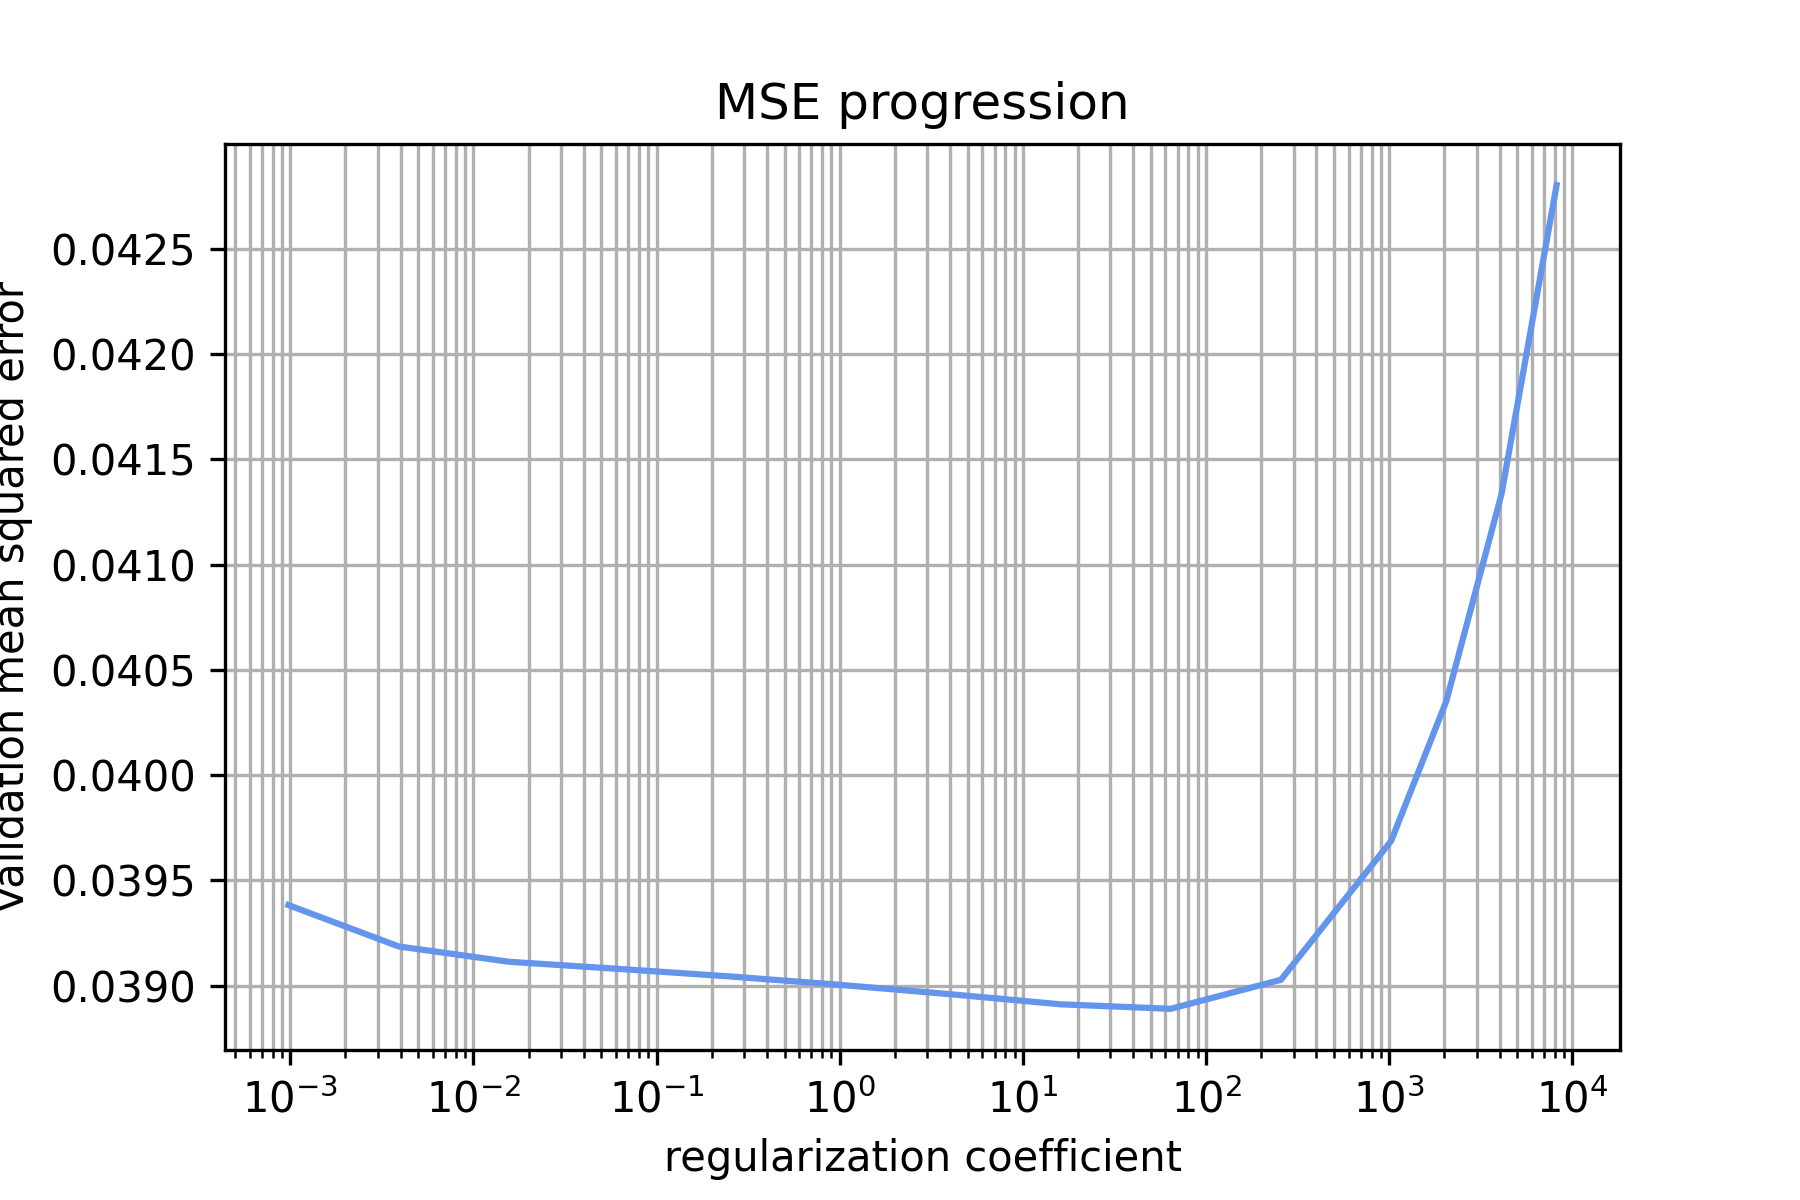
\includegraphics[width=7.5cm]{alpha_MSE_coarse_search}
        \caption{MSE progression}
        \label{fig:alpha-coarse-mse}
    \end{subfigure}
    \hfill
    % digit 1
    \begin{subfigure}{0.48\textwidth}
        \centering
        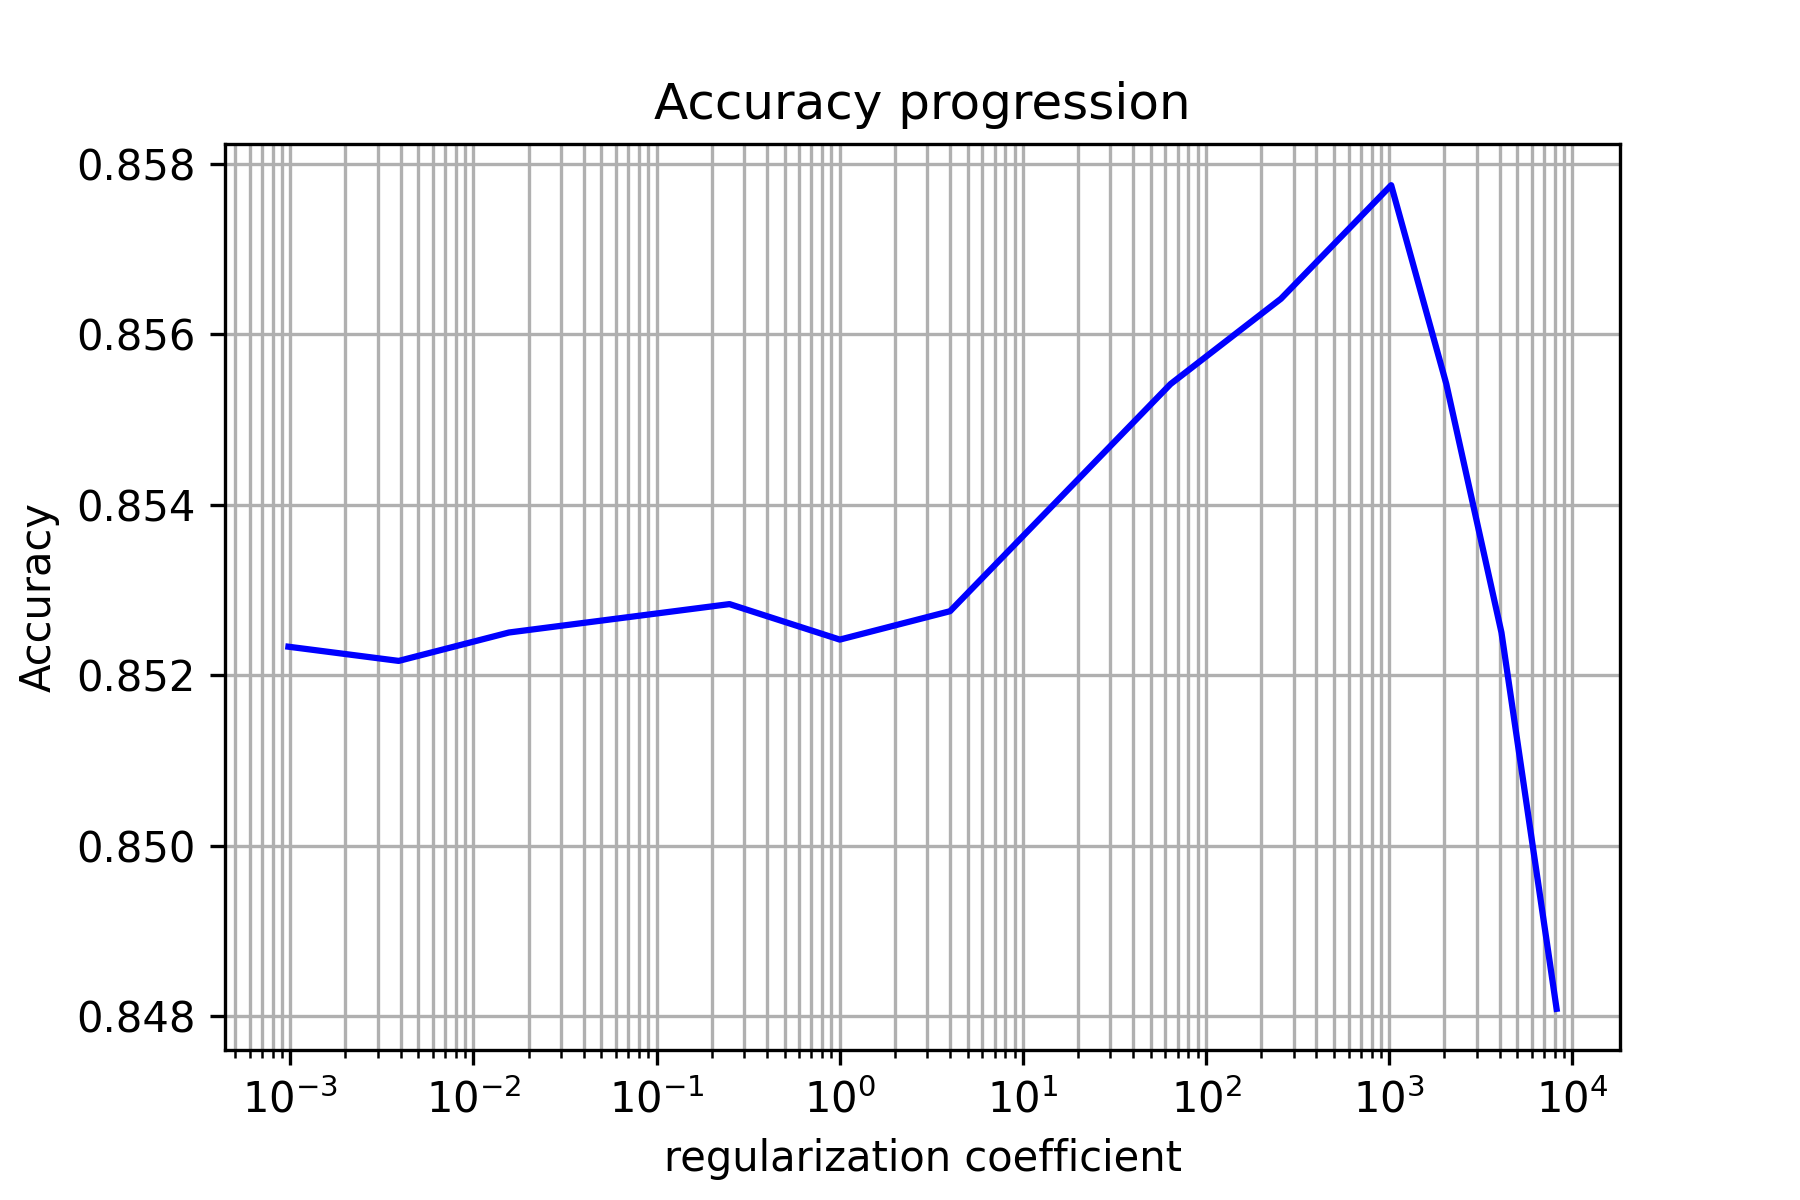
\includegraphics[width=7.5cm]{alpha_ACCURACY_coarse_search}
        \caption{Accuracy progression}
        \label{fig:alpha-coarse-acc}
    \end{subfigure}
    \hfill
    % caption and label
    \caption{Progression of MSE and accuracy in validation set for different values of the regularization coefficient (coarse search)}
    \label{fig:alpha_coarse}
\end{figure}

%=================================================
\subsection{Fine search}
%=================================================

\paragraph{In order to perform the fine search of the regularization coefficient, a golden-section one dimensional search algorithm was coded. Among the function parameters, the most important ones are the intervals of the search, precision desired and the loss function. The code can be found in:\\
\url{https://github.com/ito-rafael/machine-learning/blob/master/snippets/golden_section_search_valid.py}}

\begin{figure}[H]
    \centering
    % digit 0
    \begin{subfigure}{0.48\textwidth}
        \centering
        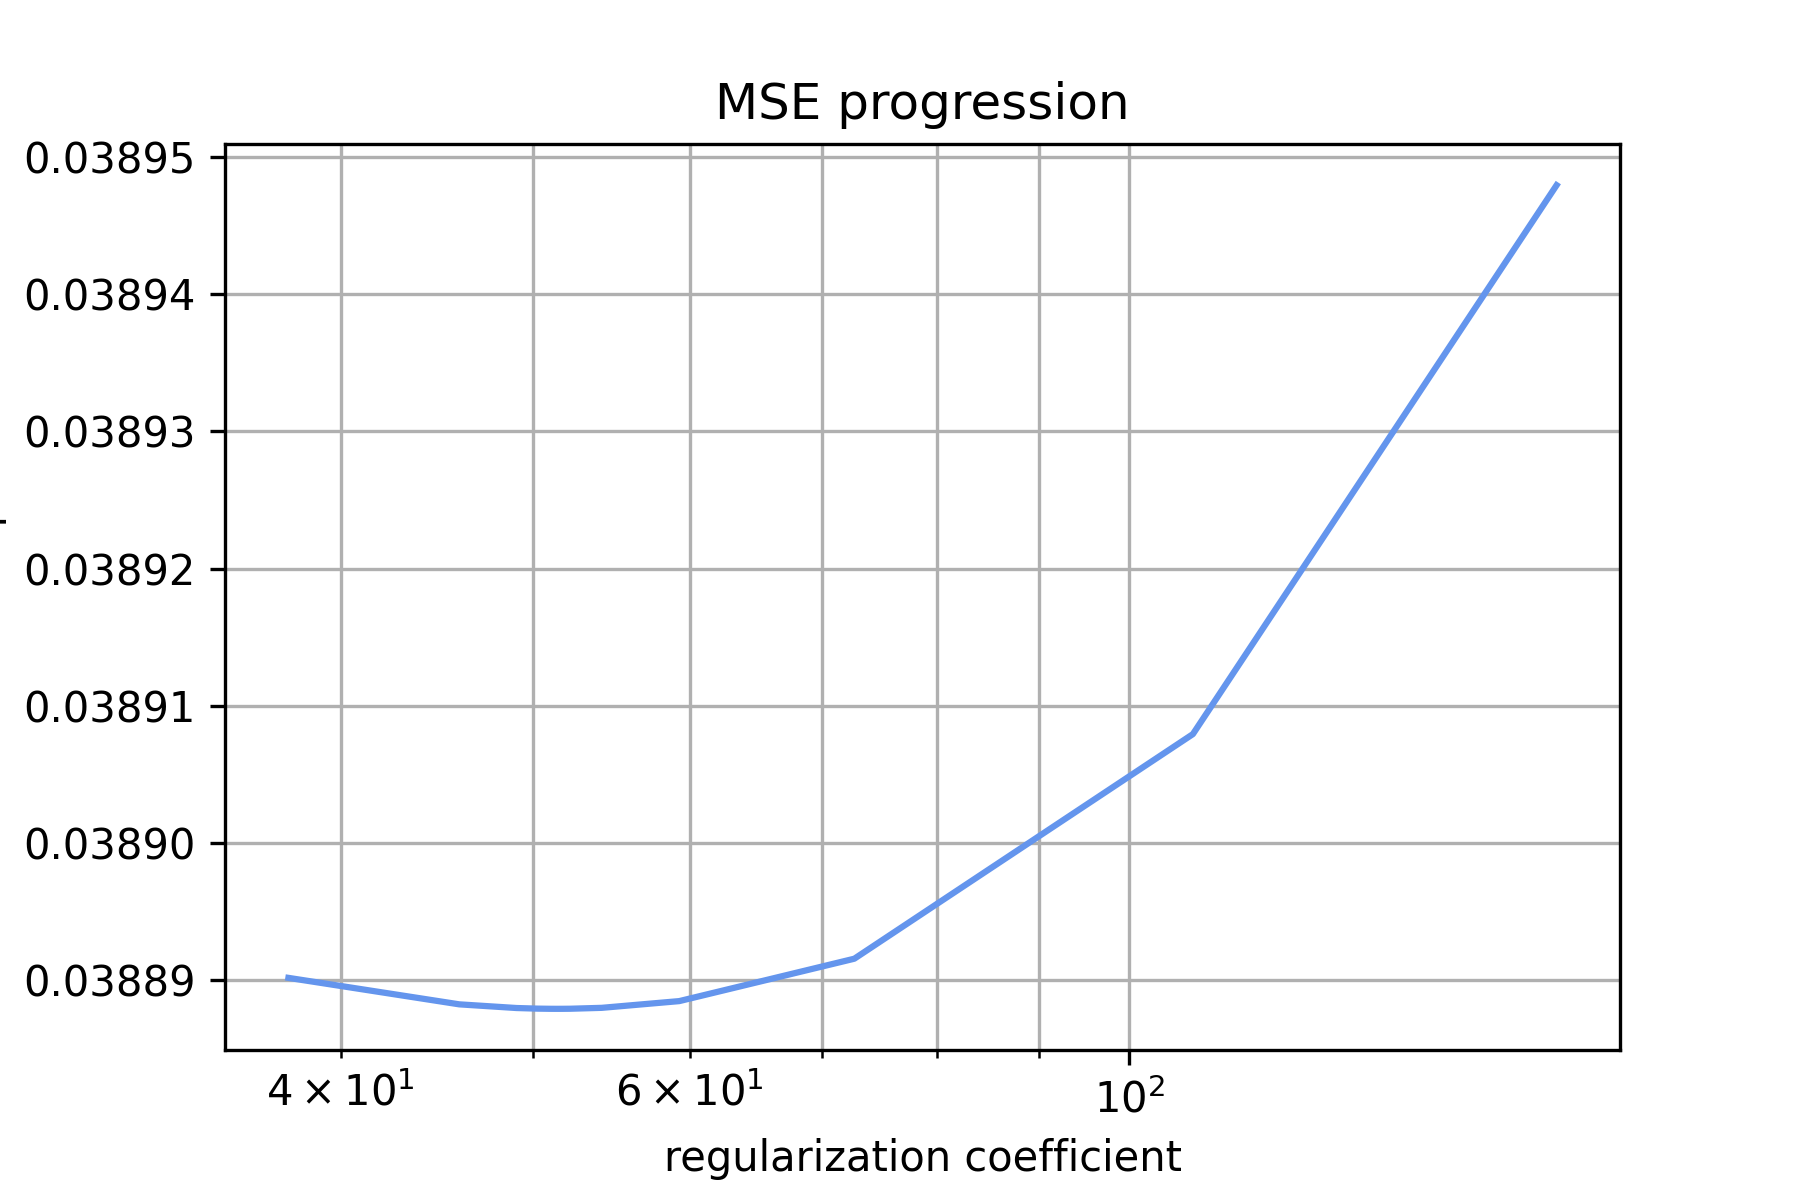
\includegraphics[width=7.5cm]{alpha_MSE_fine_search}
        \caption{MSE progression)}
        \label{fig:alpha-fine-mse}
    \end{subfigure}
    \hfill
    % digit 1
    \begin{subfigure}{0.48\textwidth}
        \centering
        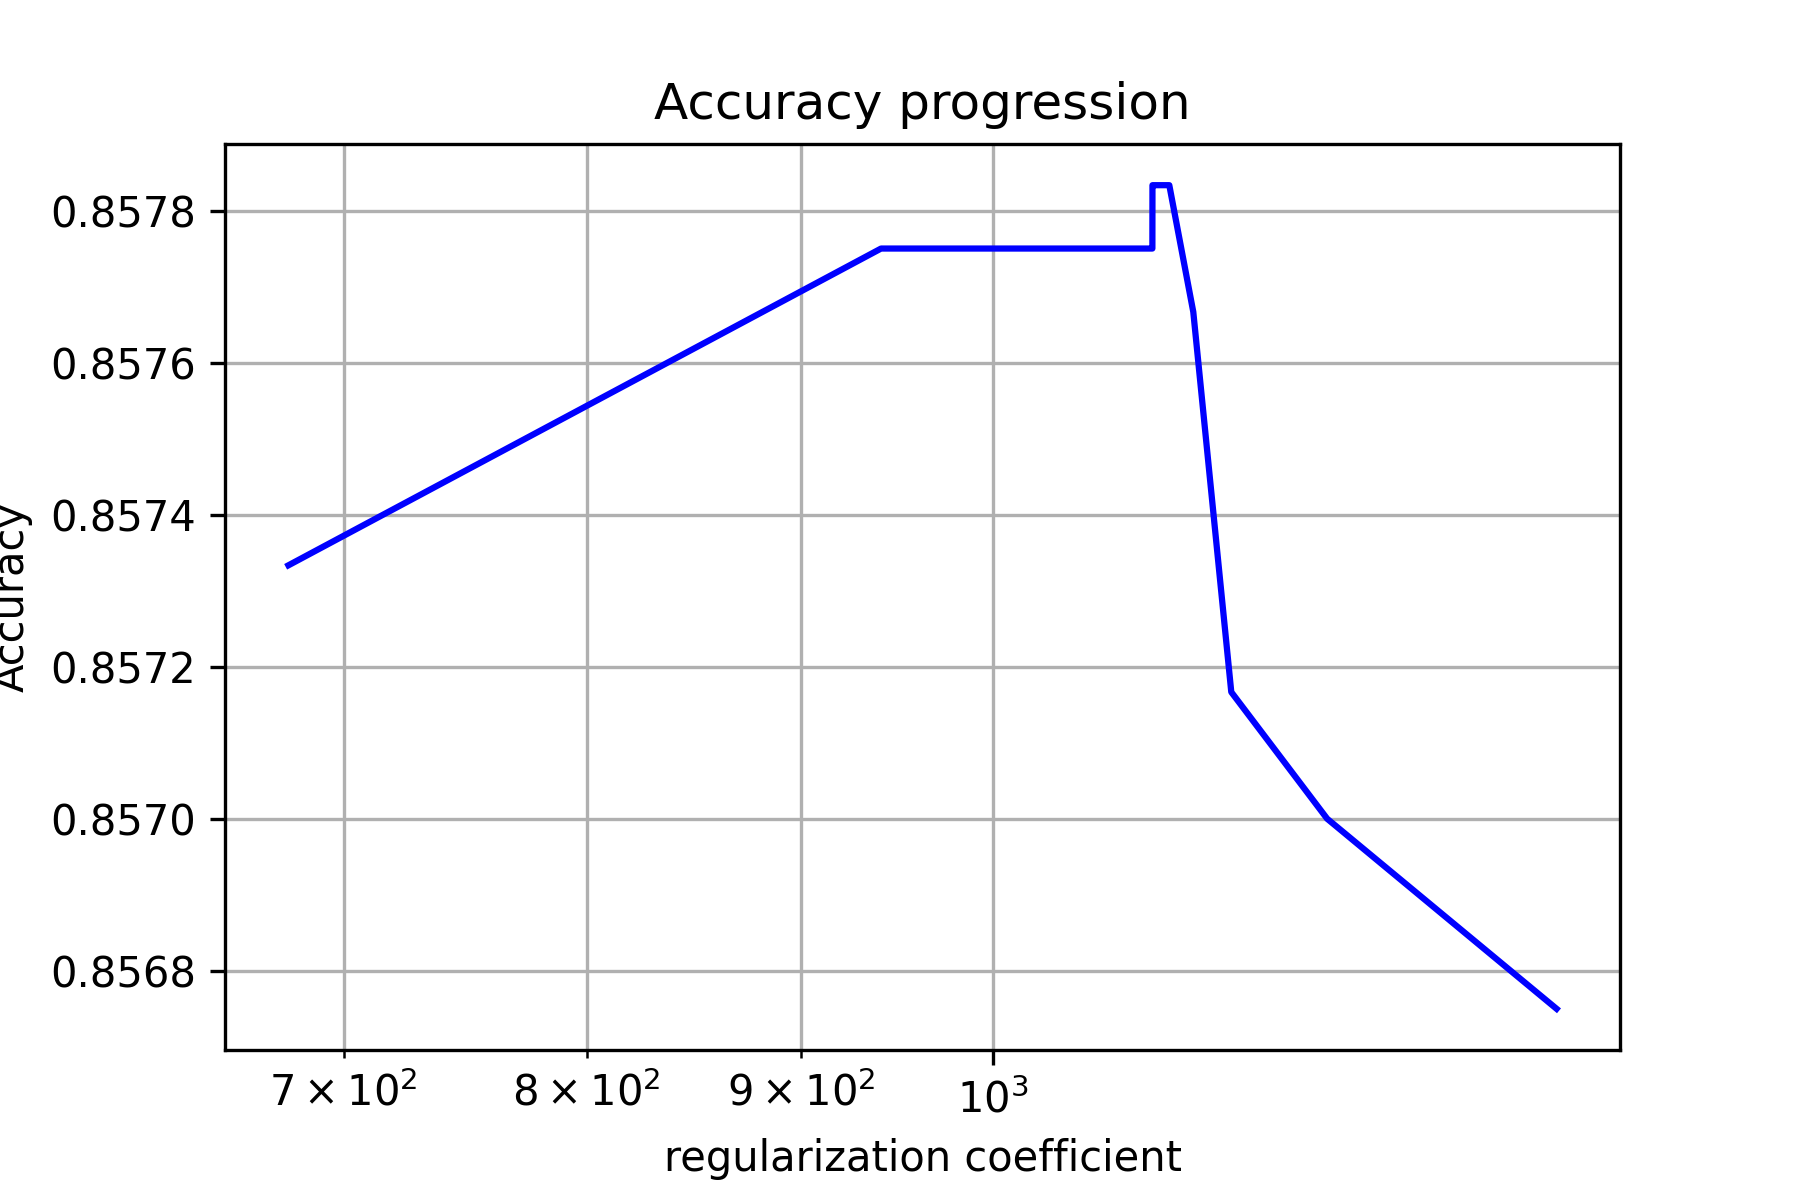
\includegraphics[width=7.5cm]{alpha_ACCURACY_fine_search}
        \caption{Accuracy progression)}
        \label{fig:alpha-fine-acc}
    \end{subfigure}
    \hfill
    % caption and label
    \caption{Progression of MSE and accuracy in validation set for different values of the regularization coefficient (fine search)}
    \label{fig:alpha_fine}
\end{figure}

%=================================================
\section{Confusion Matrix}
%=================================================

\paragraph{The values displayed in the confusion matrix were obtained with the linear classifier applied in the test set. The test set is somewhat balanced, containing the number of samples for each class as illustrated in Figure \ref{tab:samples_test_set}}

\begin{table}[H]
    \begin{center}
        \begin{tabular}{|c|c|} 
            \cline{1-2}
            \cellcolor[gray]{0.8}{Digit} & \cellcolor[gray]{0.8}{nº of samples} \\
            \cline{1-2}
            0 &  980 \\
            1 & 1135 \\
            2 & 1032 \\
            3 & 1010 \\
            4 &  982 \\
            5 &  892 \\
            6 &  958 \\
            7 & 1028 \\
            8 &  974 \\
            9 & 1009 \\
            \cline{1-2}
        \end{tabular}
    \end{center}
    \caption{Number of samples for each class in the test set}
    \label{tab:samples_test_set}
\end{table}

\begin{figure}[H]
    \centering
    % digit 0
    \begin{subfigure}{0.48\textwidth}
        \centering
        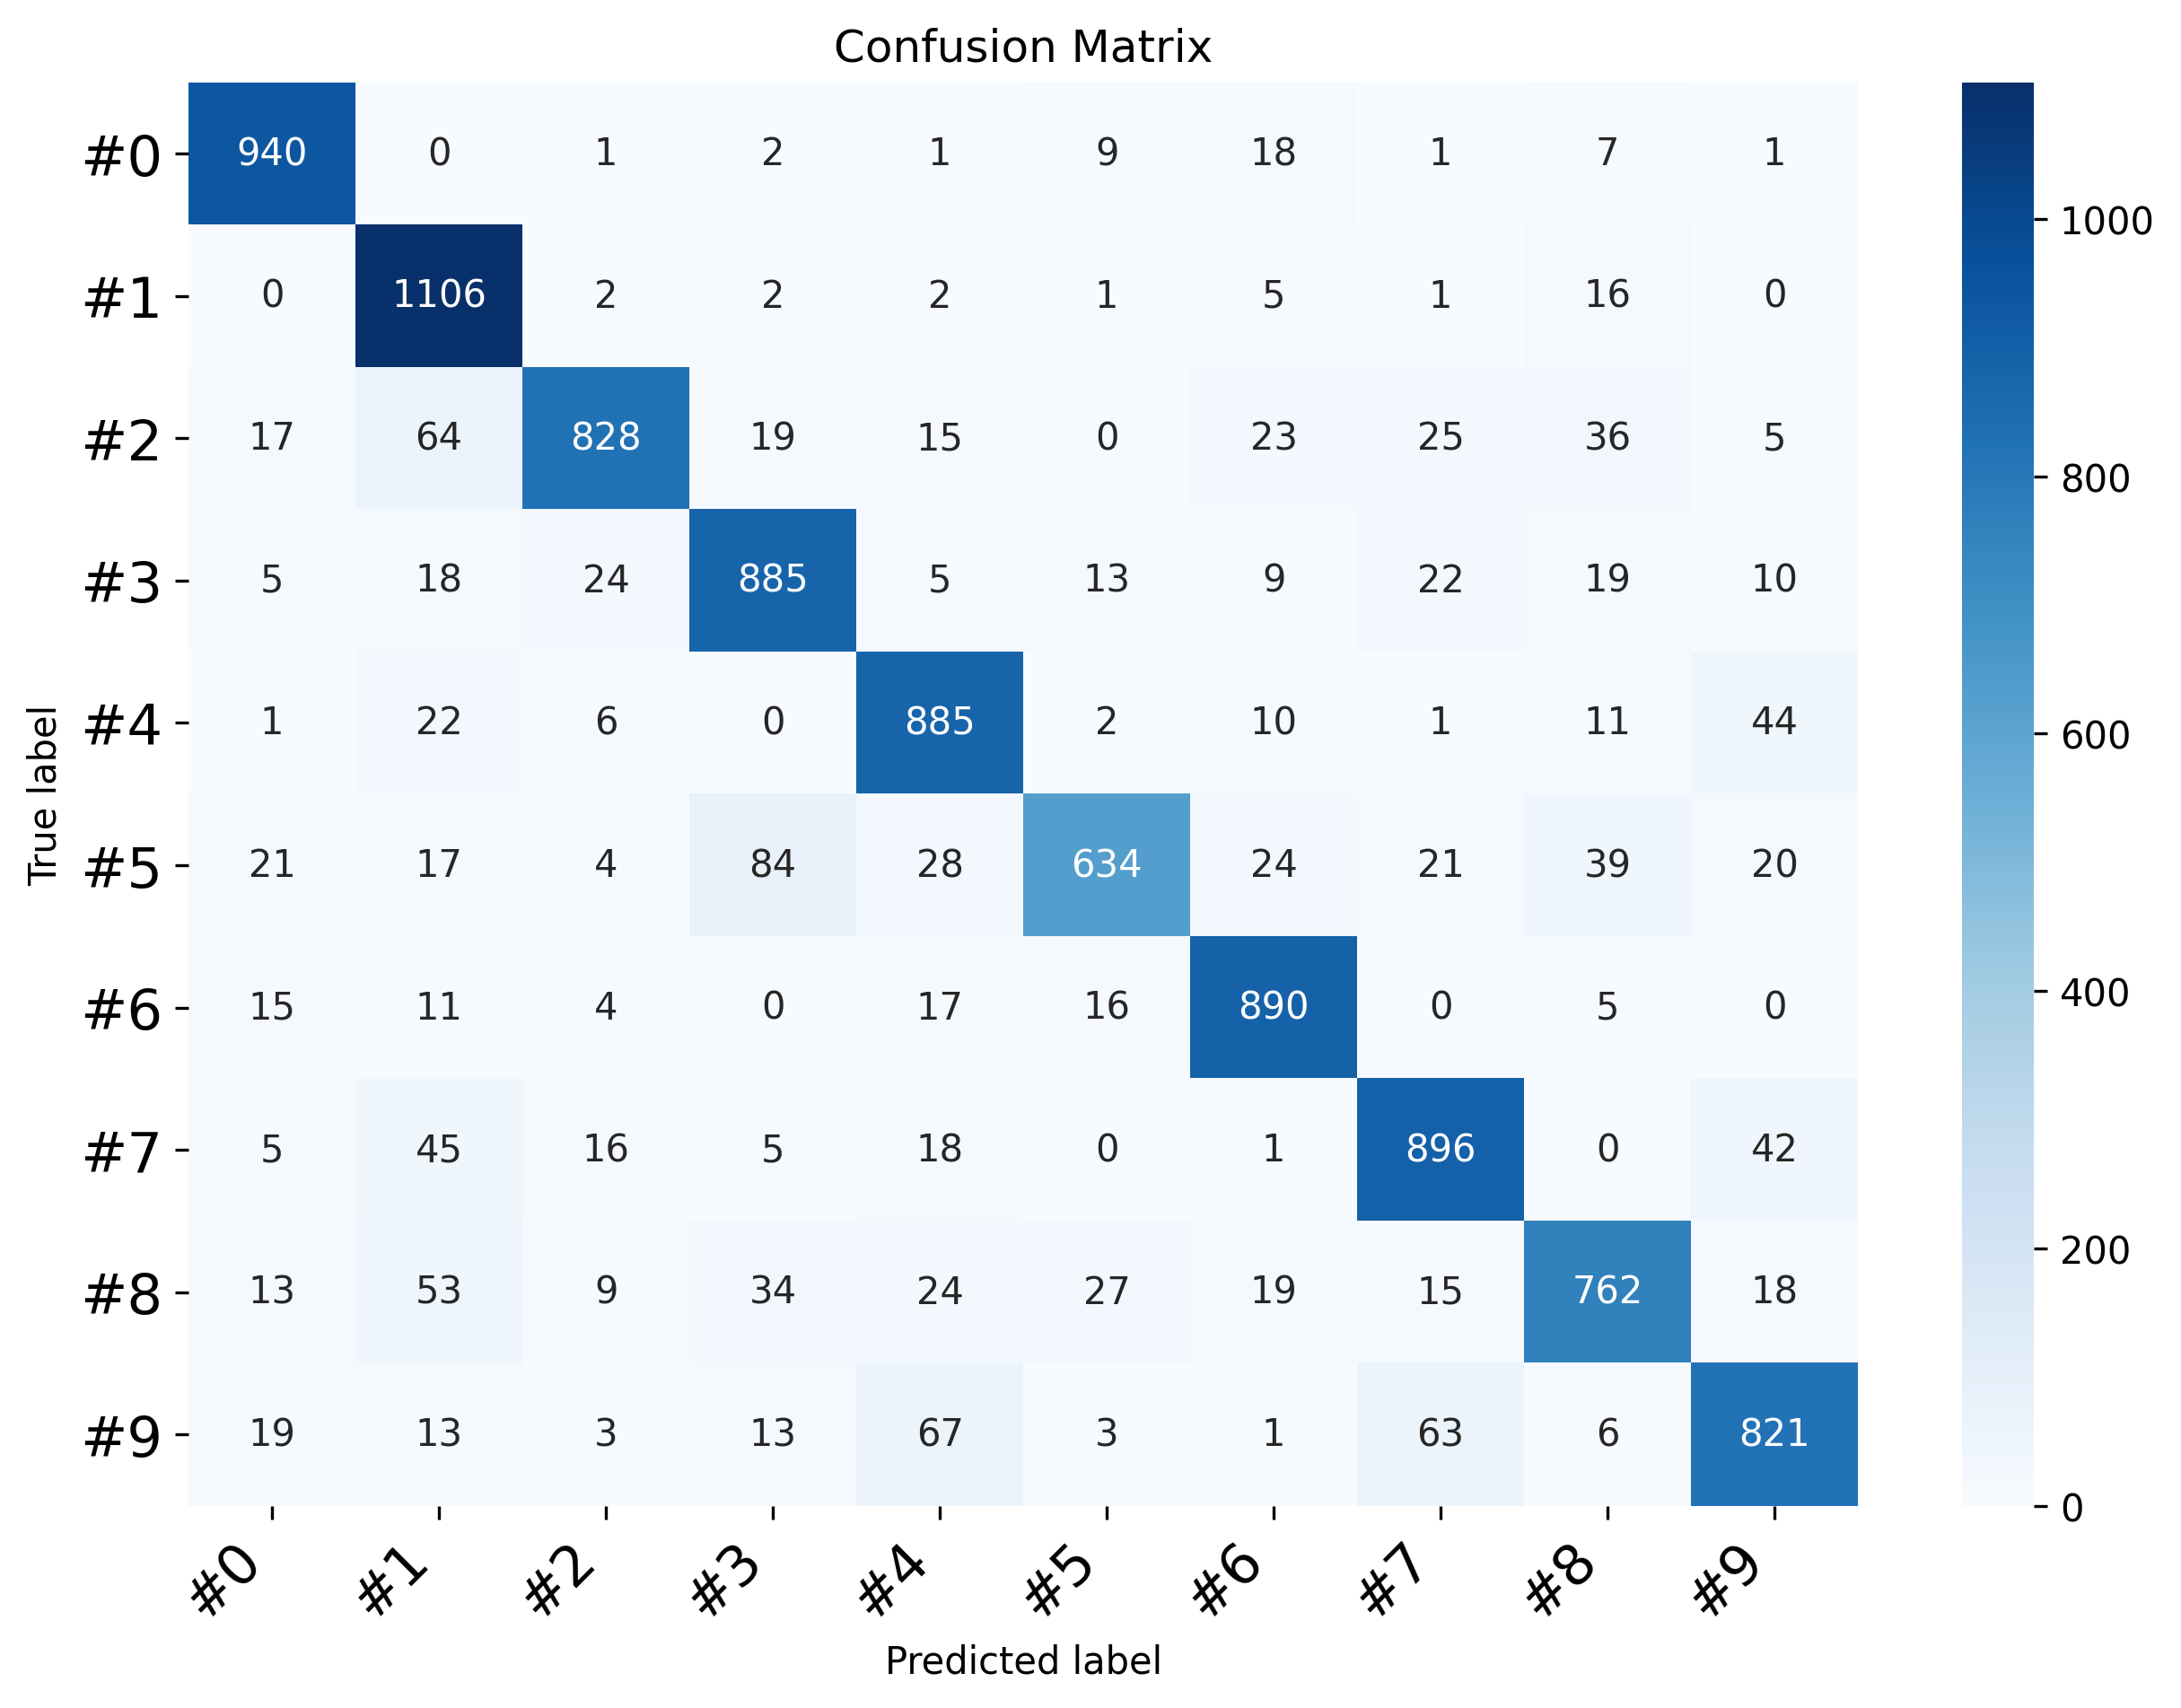
\includegraphics[width=7.5cm]{cm_raw}
        \caption{Confusion matrix with raw values}
        \label{fig:cm_raw}
    \end{subfigure}
    \hfill
    % digit 1
    \begin{subfigure}{0.48\textwidth}
        \centering
        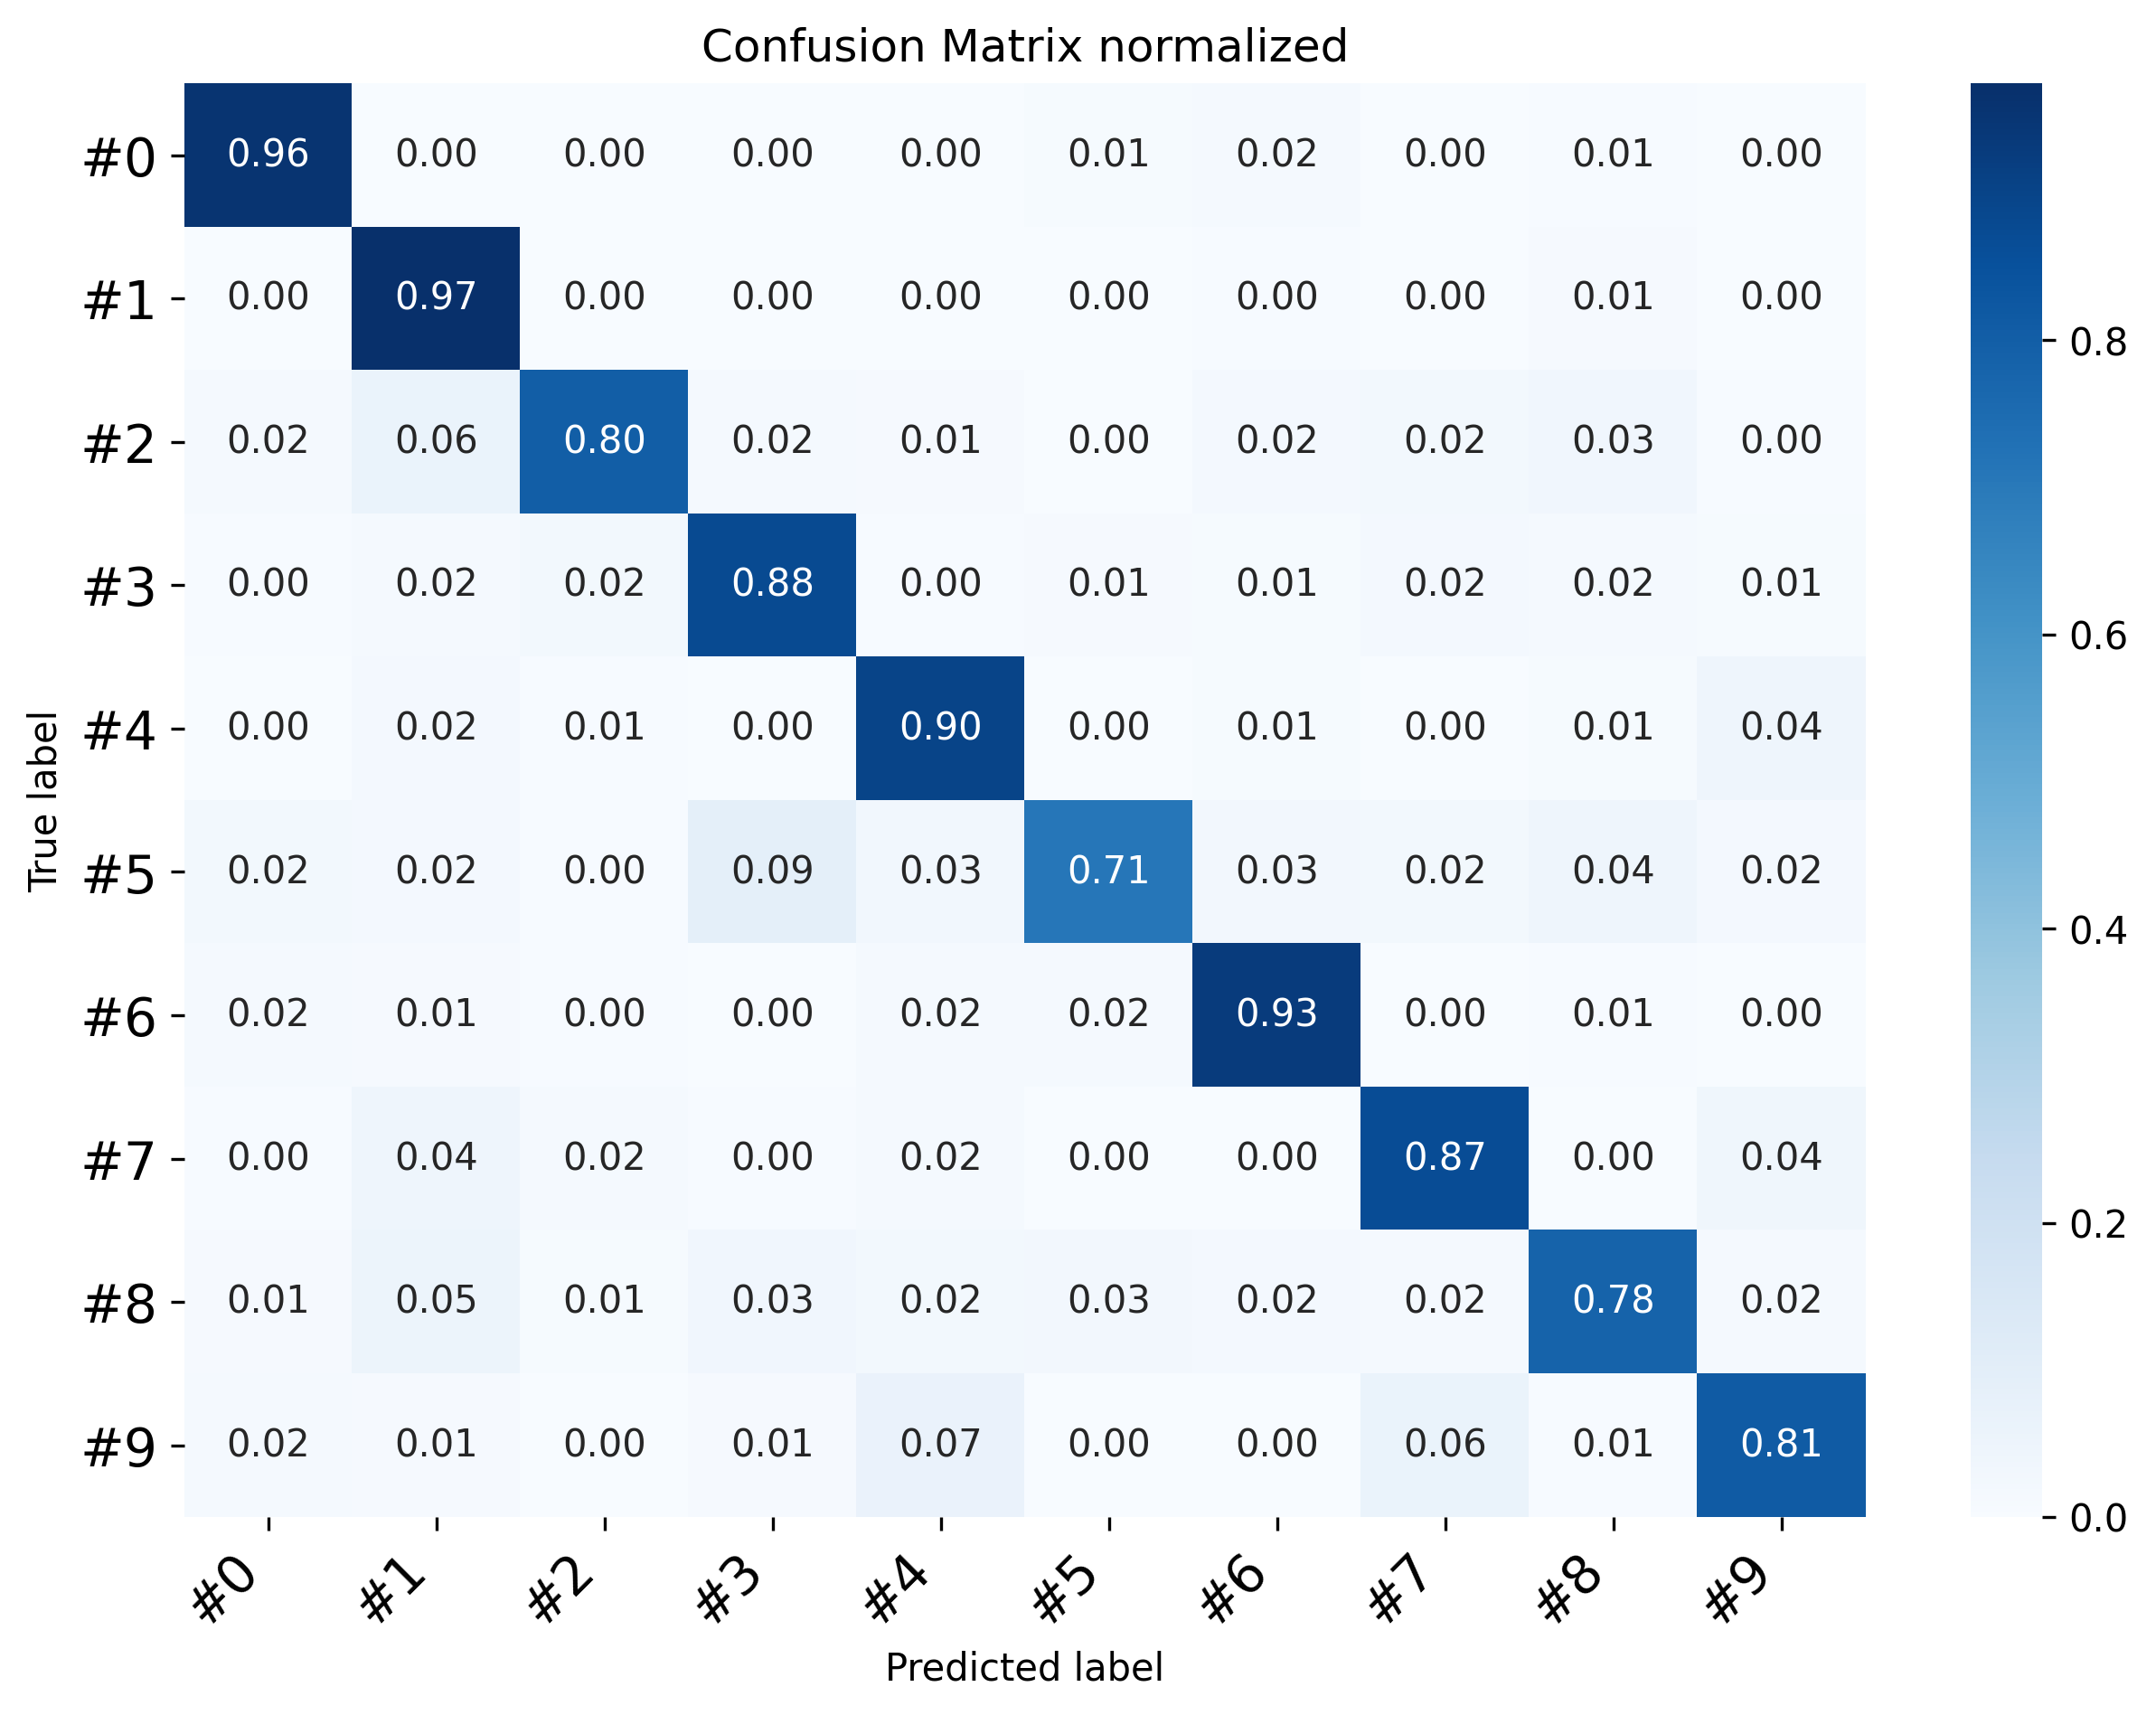
\includegraphics[width=7.5cm]{cm_norm}
        \caption{Confusion matrix with normalized values}
        \label{fig:cm_norm}
    \end{subfigure}
    \hfill
    % caption and label
    \caption{Confusion matrix with normalized and raw values} 
    \label{fig:cm}
\end{figure}

%=================================================
\section{Classifier Heatmap}
%=================================================

\begin{figure}[H]
    \centering
    % digit 1
    \begin{subfigure}{0.24\textwidth}
        \centering
        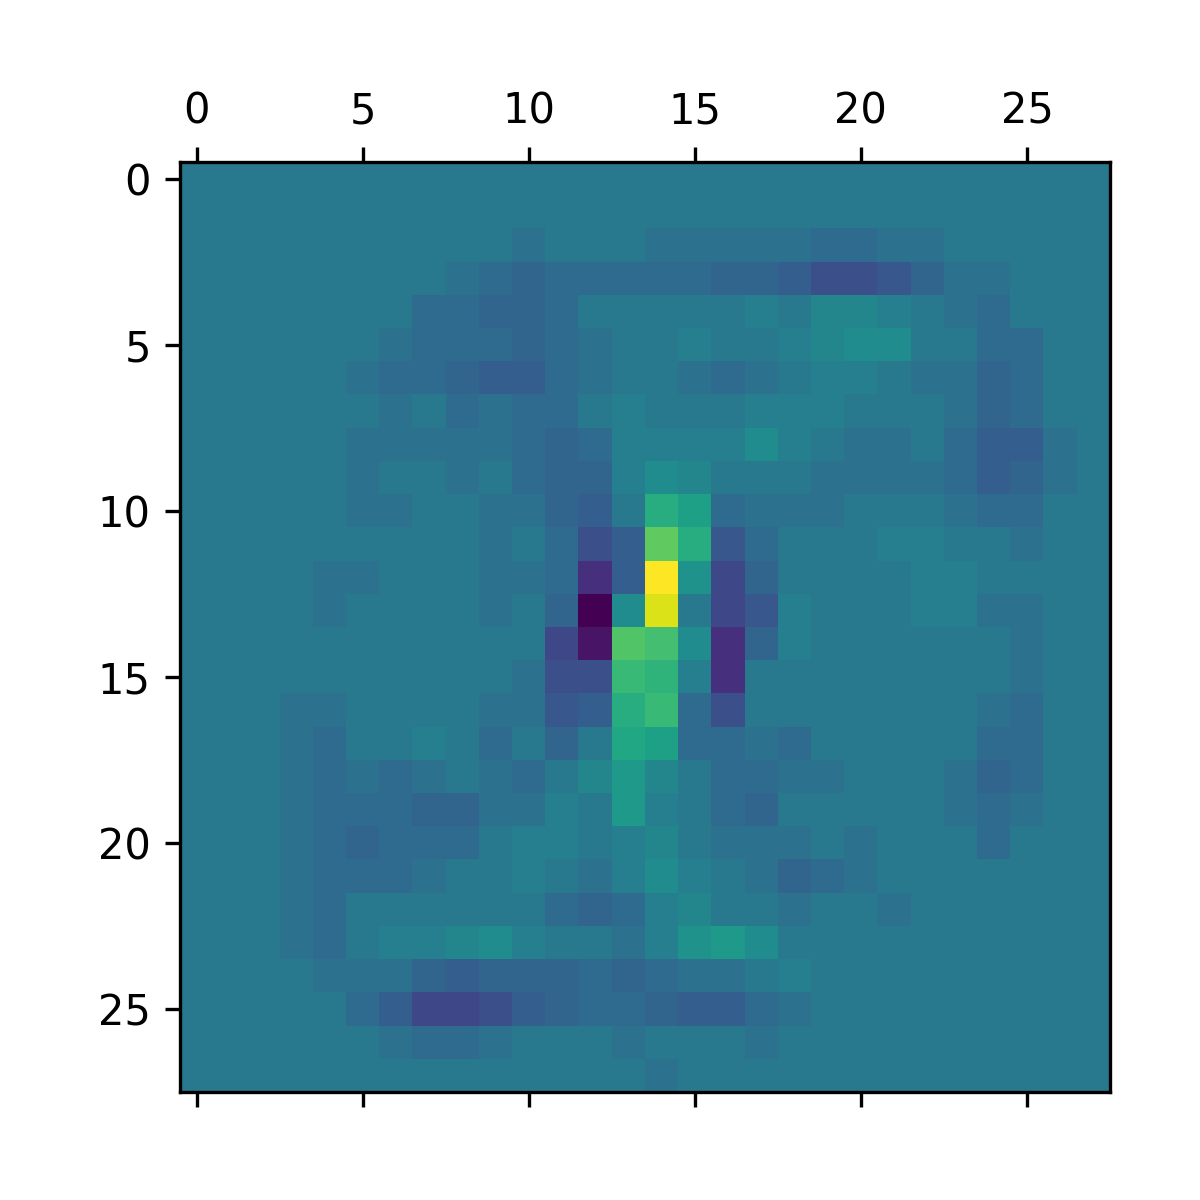
\includegraphics[width=3.5cm]{digit_1}
        \caption{Digit 1 heatmap}
        \label{fig:digit_1}
    \end{subfigure}
    \hfill
    % digit 2
    \begin{subfigure}{0.24\textwidth}
        \centering
        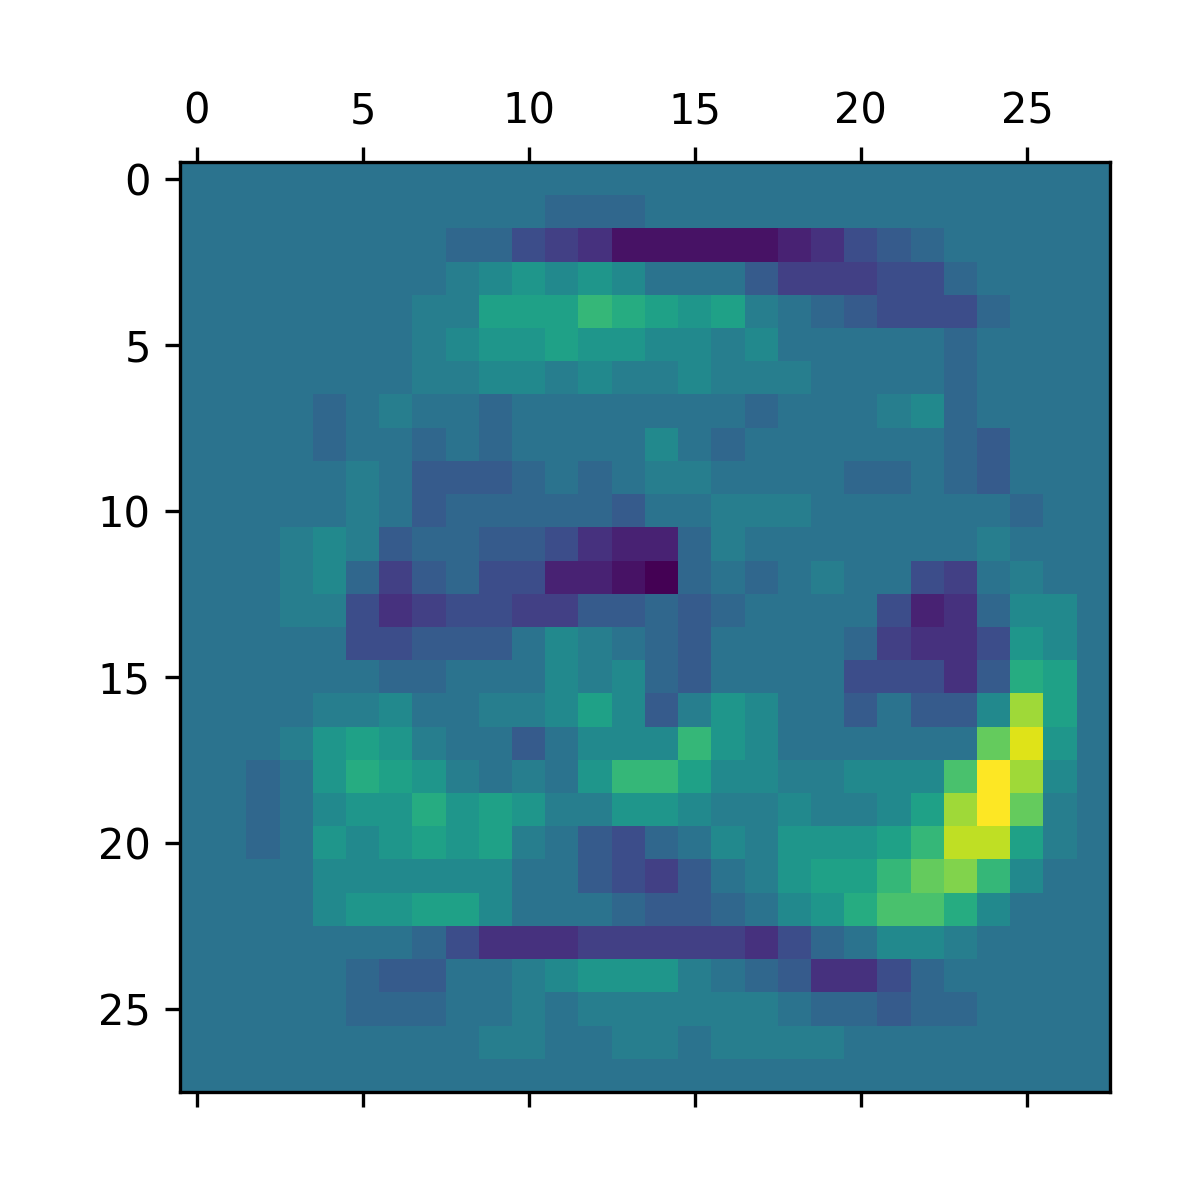
\includegraphics[width=3.5cm]{digit_2}
        \caption{Digit 2 heatmap}
        \label{fig:digit_2}
    \end{subfigure}
    \hfill
    % digit 3
    \begin{subfigure}{0.24\textwidth}
        \centering
        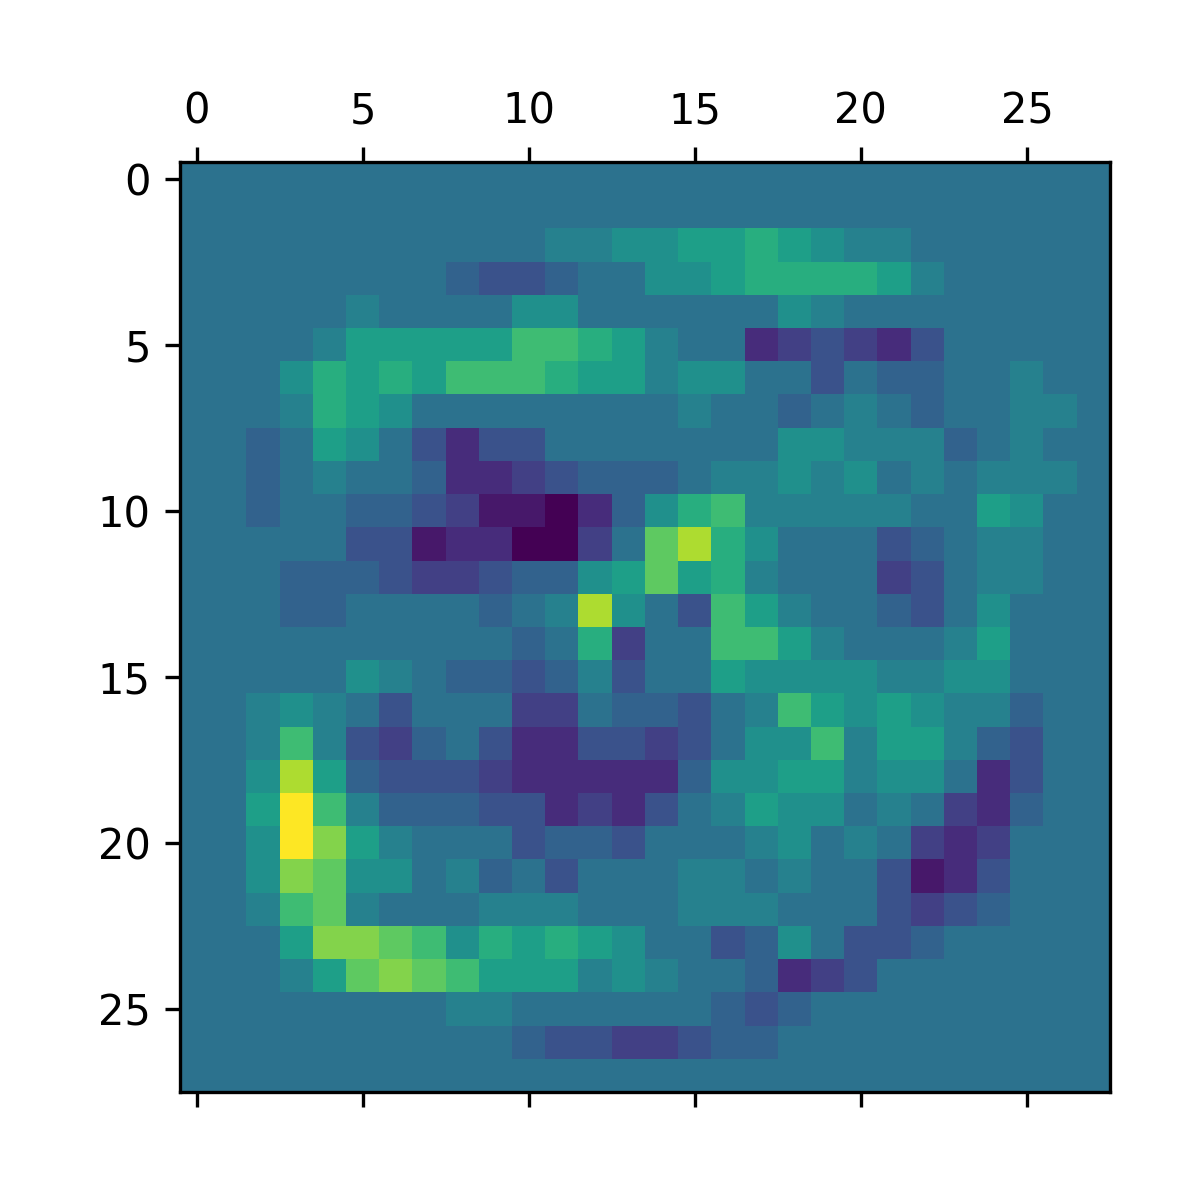
\includegraphics[width=3.5cm]{digit_3}
        \caption{Digit 3 heatmap}
        \label{fig:digit_3}
    \end{subfigure}
    \hfill
    % digit 4
    \begin{subfigure}{0.24\textwidth}
        \centering
        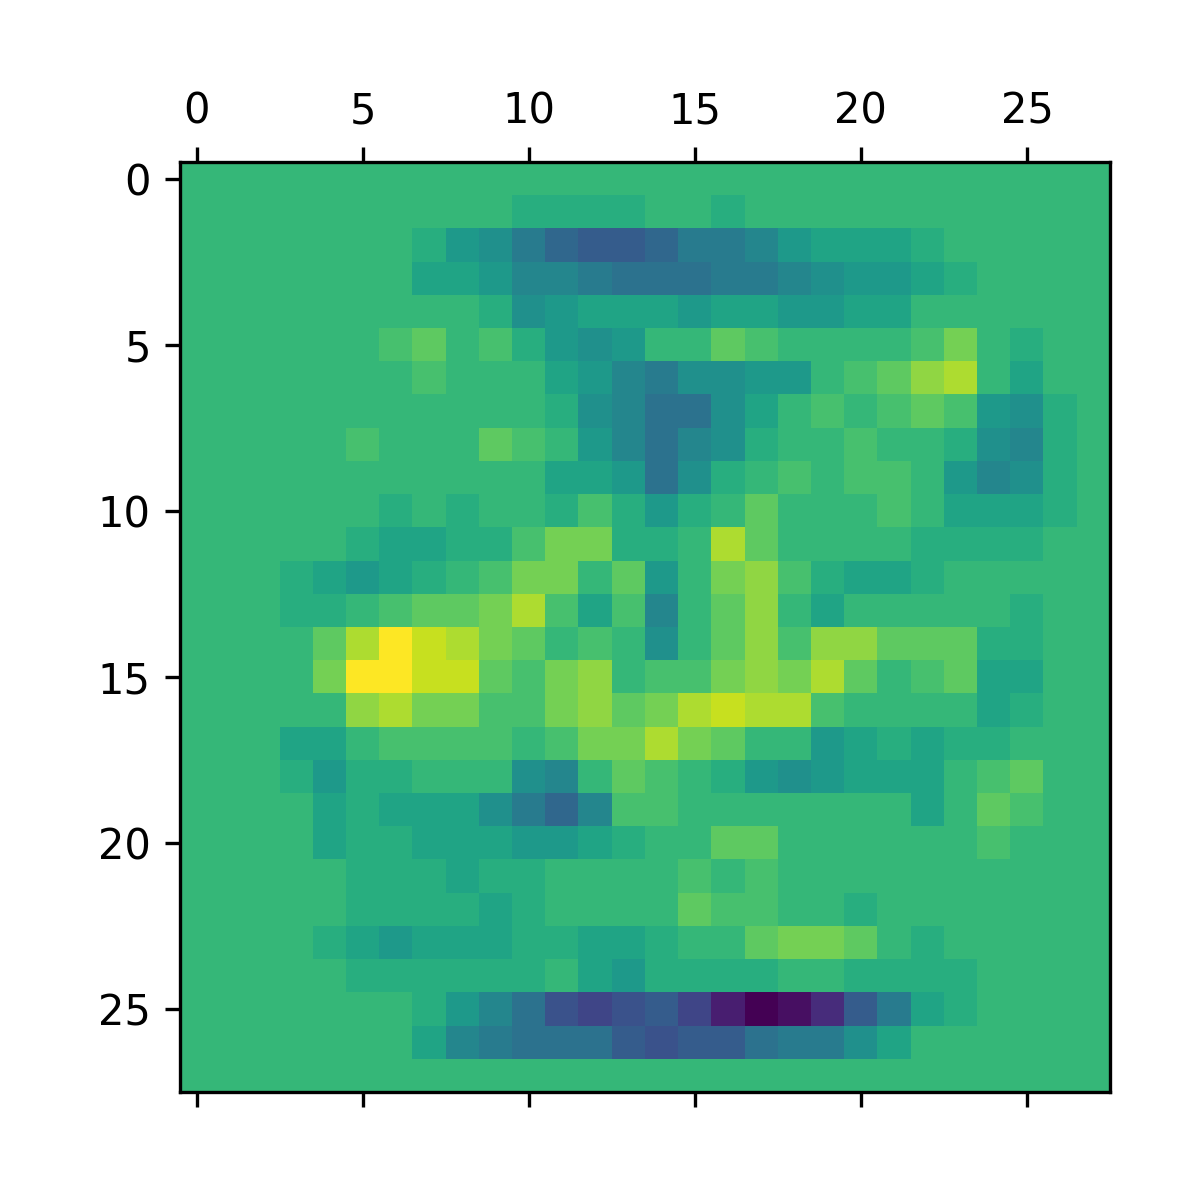
\includegraphics[width=3.5cm]{digit_4}
        \caption{Digit 4 heatmap}
        \label{fig:digit_4}
    \end{subfigure}
    \hfill
    % digit 5
    \begin{subfigure}{0.24\textwidth}
        \centering
        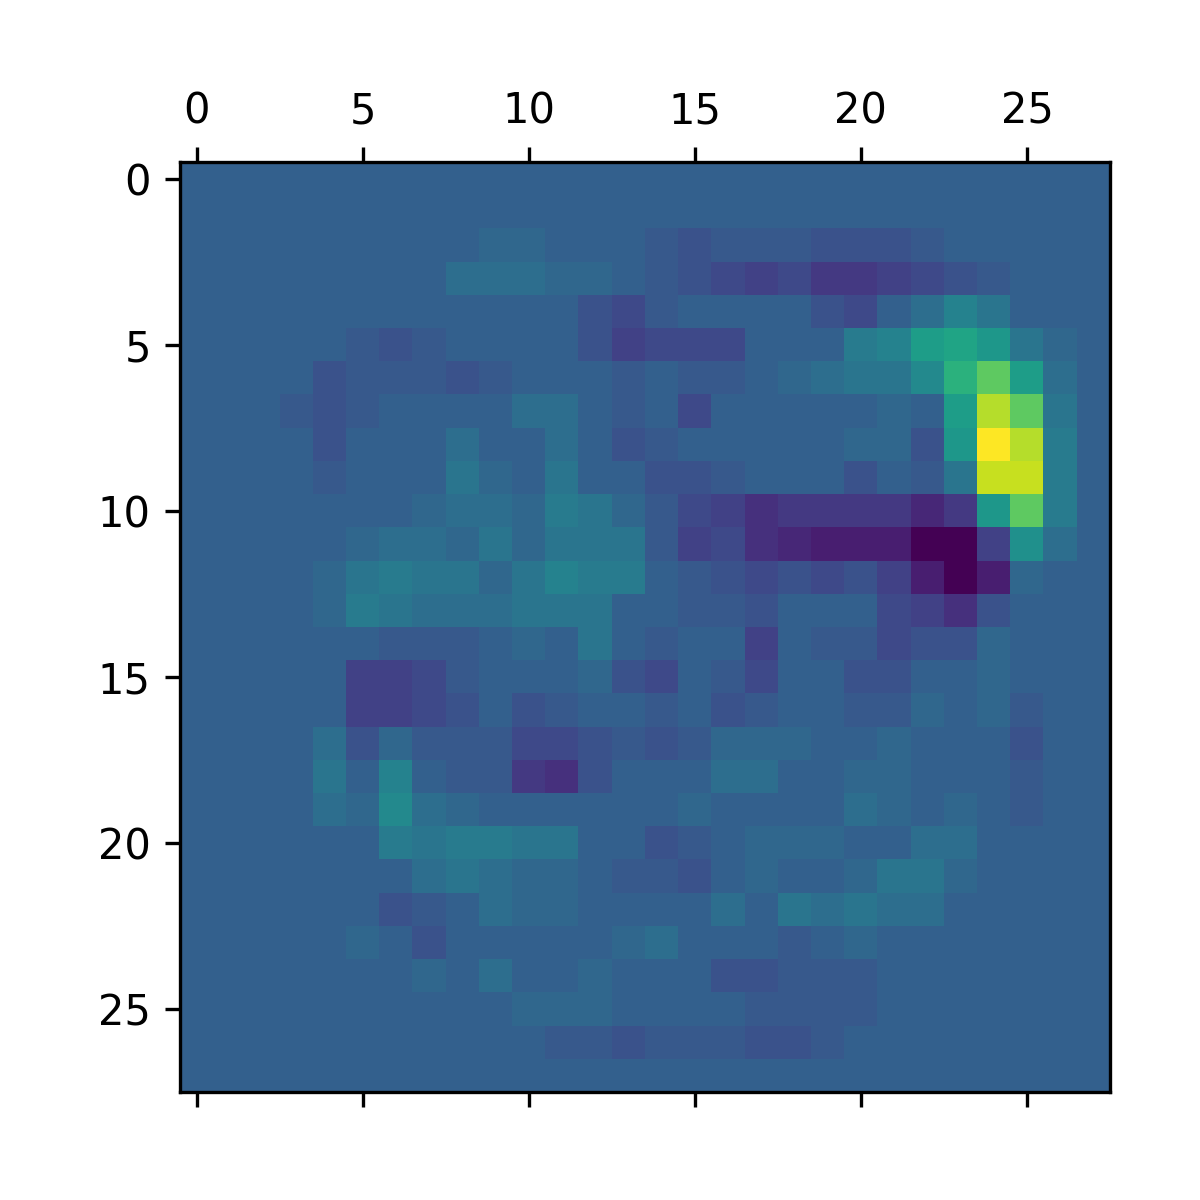
\includegraphics[width=3.5cm]{digit_5}
        \caption{Digit 5 heatmap}
        \label{fig:digit_5}
    \end{subfigure}
    \hfill
    % digit 6
    \begin{subfigure}{0.24\textwidth}
        \centering
        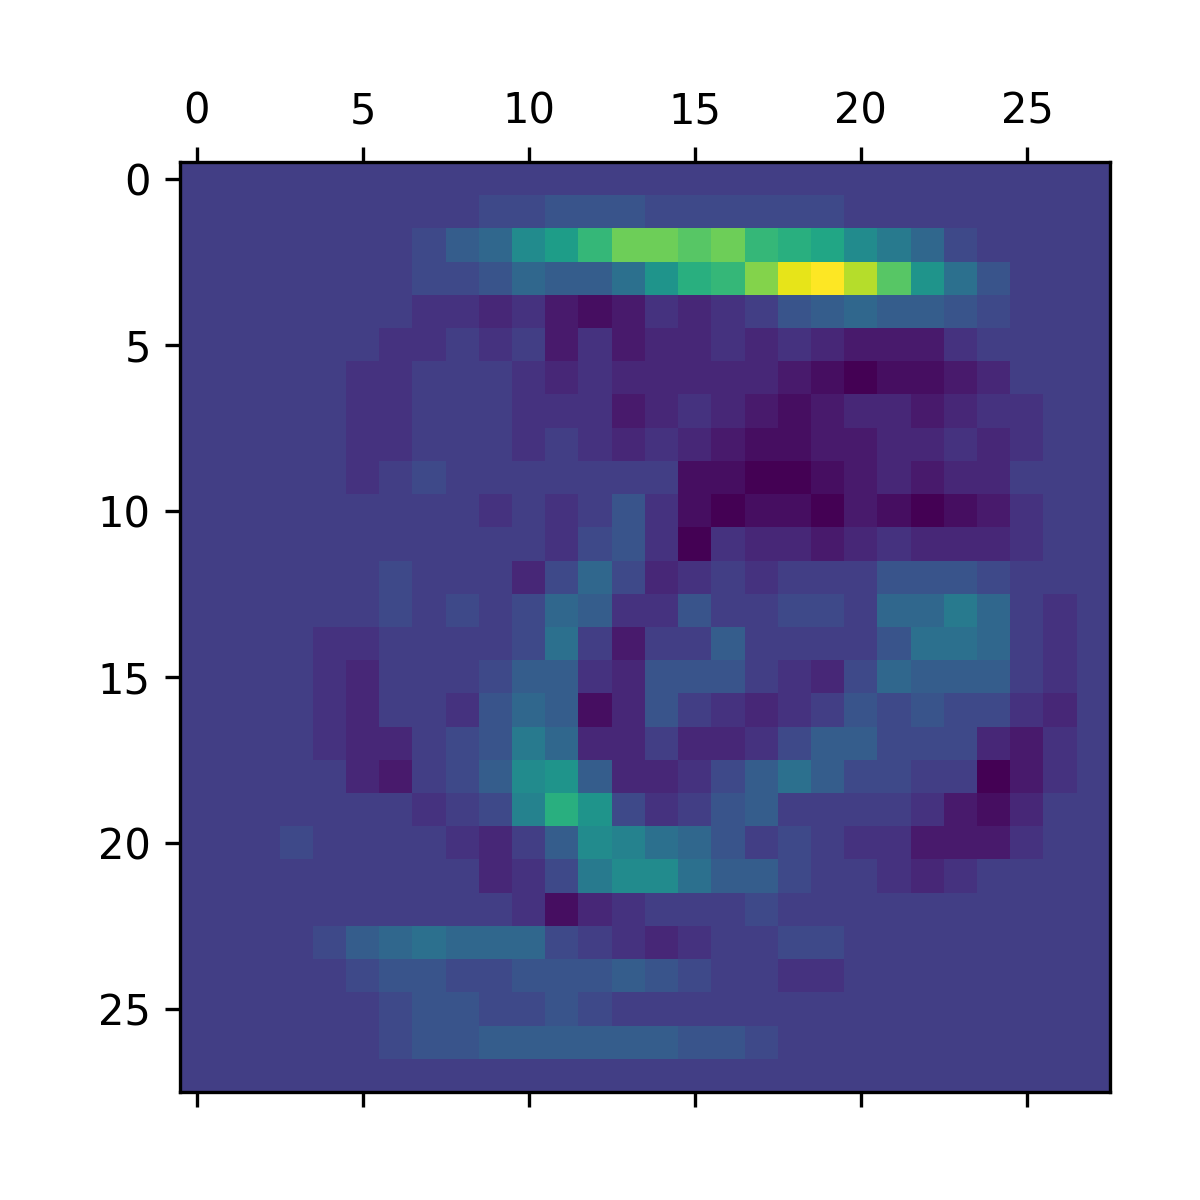
\includegraphics[width=3.5cm]{digit_6}
        \caption{Digit 6 heatmap}
        \label{fig:digit_6}
    \end{subfigure}
    \hfill
    % digit 7
    \begin{subfigure}{0.24\textwidth}
        \centering
        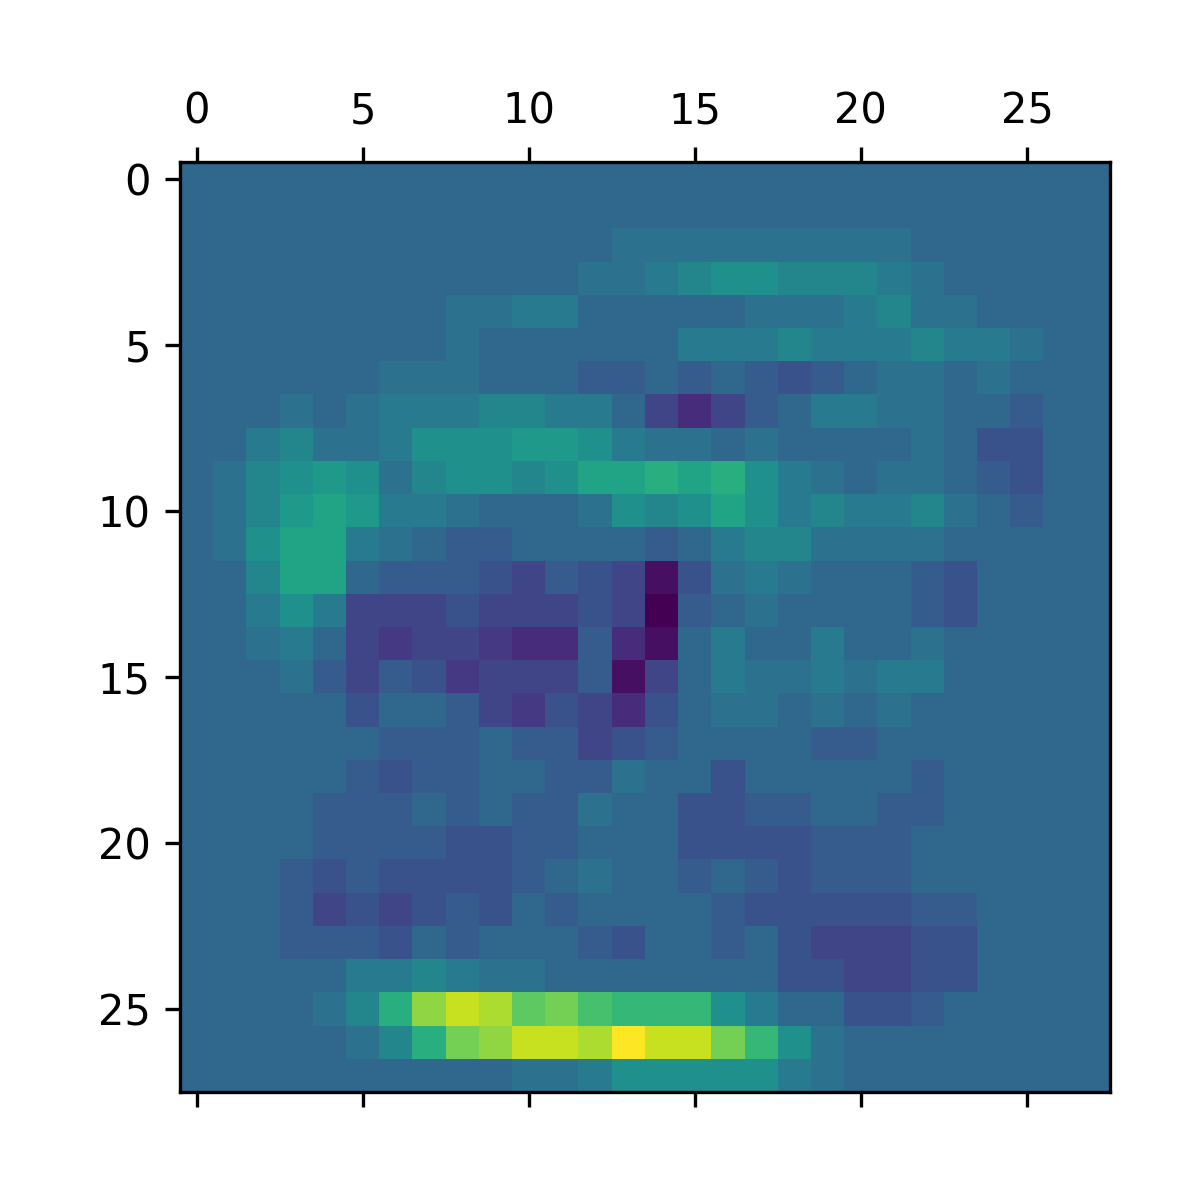
\includegraphics[width=3.5cm]{digit_7}
        \caption{Digit 7 heatmap}
        \label{fig:digit_7}
    \end{subfigure}
    \hfill
    % digit 8
    \begin{subfigure}{0.24\textwidth}
        \centering
        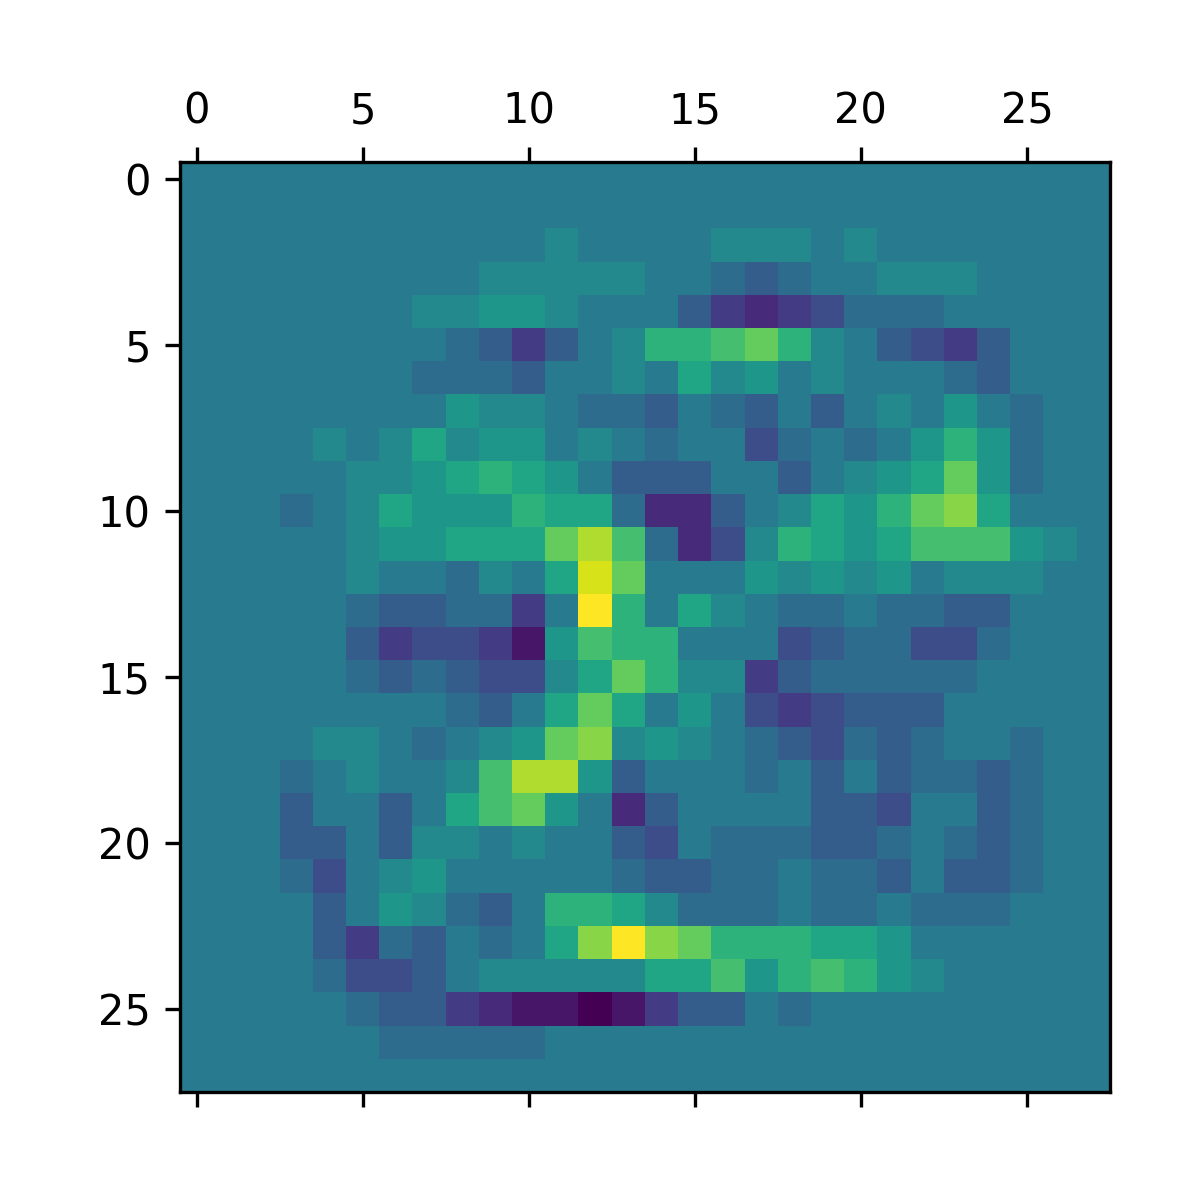
\includegraphics[width=3.5cm]{digit_8}
        \caption{Digit 8 heatmap}
        \label{fig:digit_8}
    \end{subfigure}
    \hfill
    % digit 9
    \begin{subfigure}{0.24\textwidth}
        \centering
        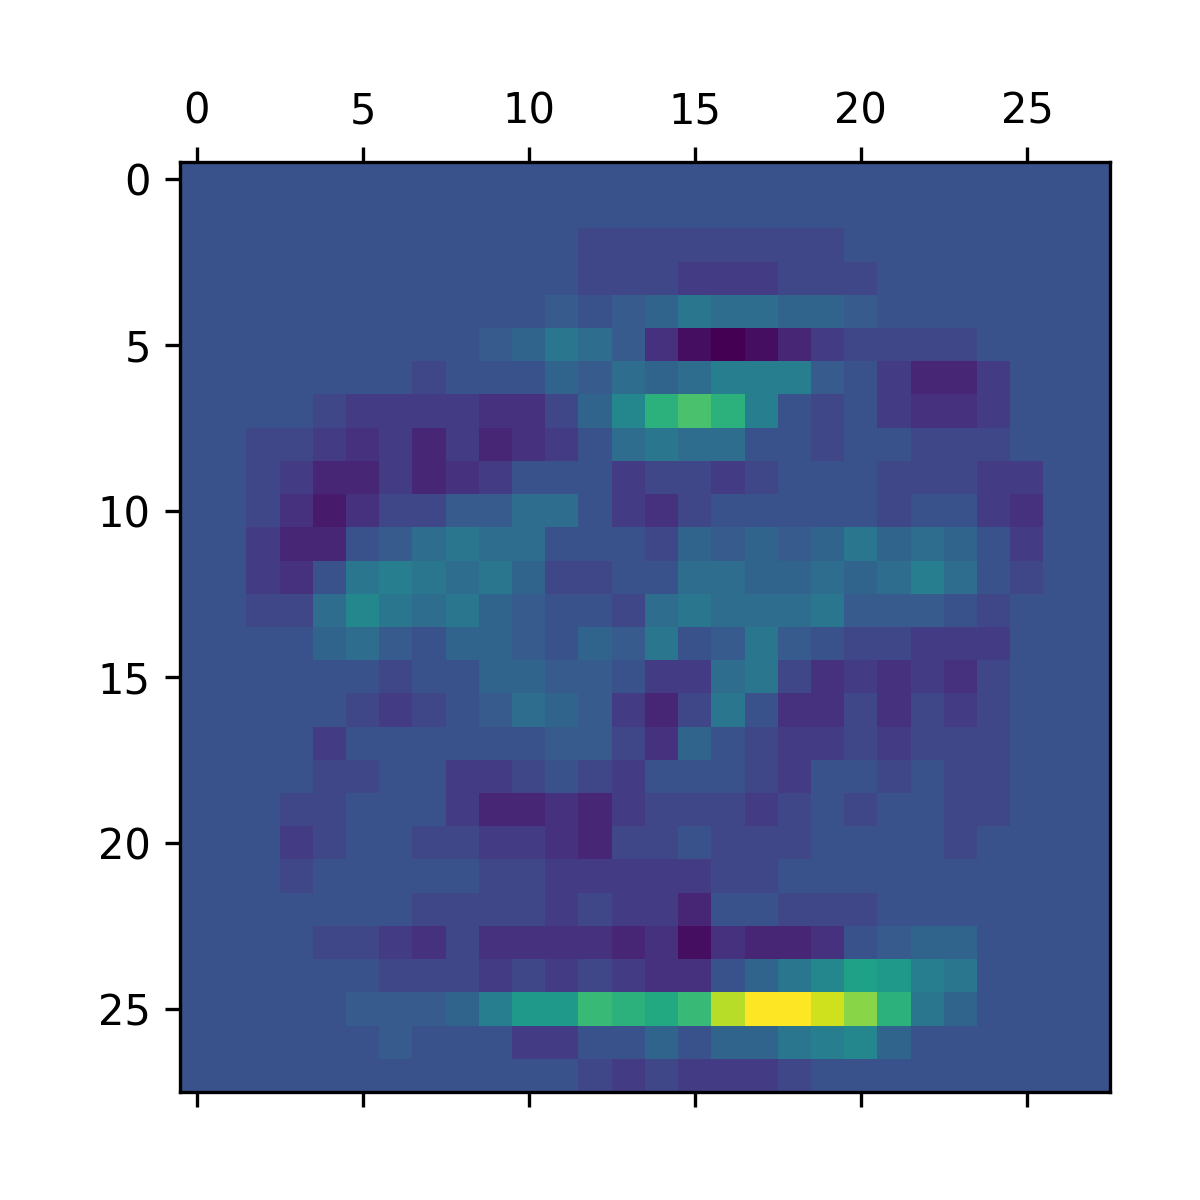
\includegraphics[width=3.5cm]{digit_9}
        \caption{Digit 9 heatmap}
        \label{fig:digit_9}
    \end{subfigure}
    \hfill
    % digit 0
    \begin{subfigure}{0.24\textwidth}
        \centering
        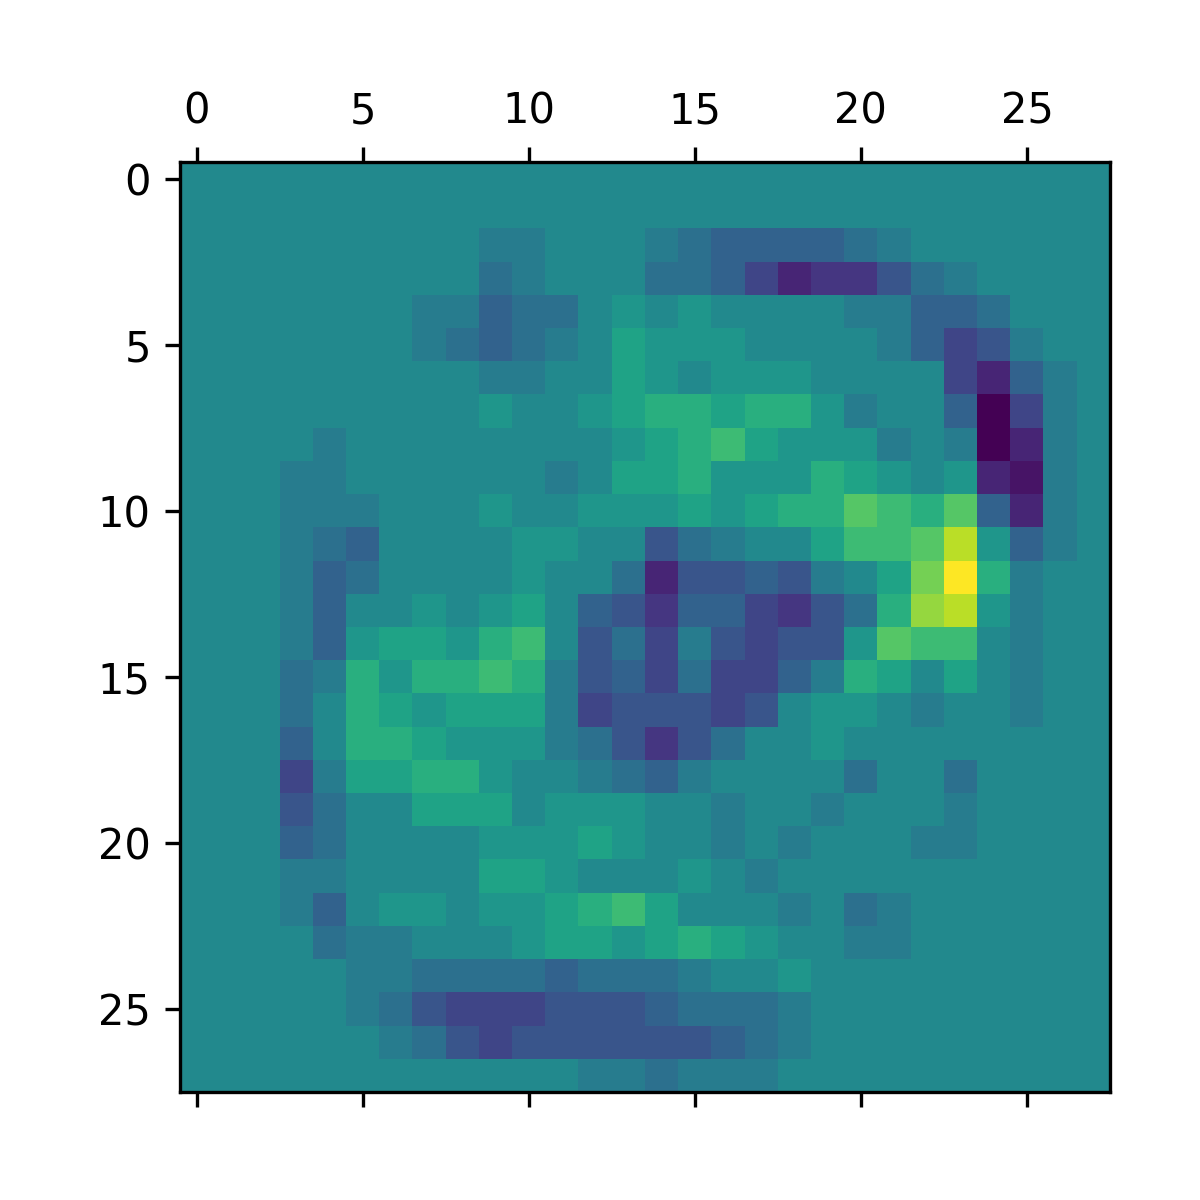
\includegraphics[width=3.5cm]{digit_0}
        \caption{Digit 0 heatmap}
        \label{fig:digit_0}
    \end{subfigure}
    \hfill
    \hspace{3.5cm}
    \hfill
    \hspace{3.5cm}
    % caption and label
    \caption{Heatmap for the classifiers correspondent to each digit} 
    \label{fig:heatmap_digits}
\end{figure}
%-------------------------------------------------

%=================================================
\section{Misclassified data}
%=================================================

\paragraph{The digits shown in Figure \ref{fig:misclassified_digits} are in the top 30 misclassified digits from which the difference between the output for the real class and the output for the predicted class are the highest. Both real and predicted class and its outputs values associated are indicated. The output is shown in parenthesis, in front of the correspondent class.}

\begin{figure}[H]
    \centering
    % example 1
    \begin{subfigure}{0.32\textwidth}
        \centering
        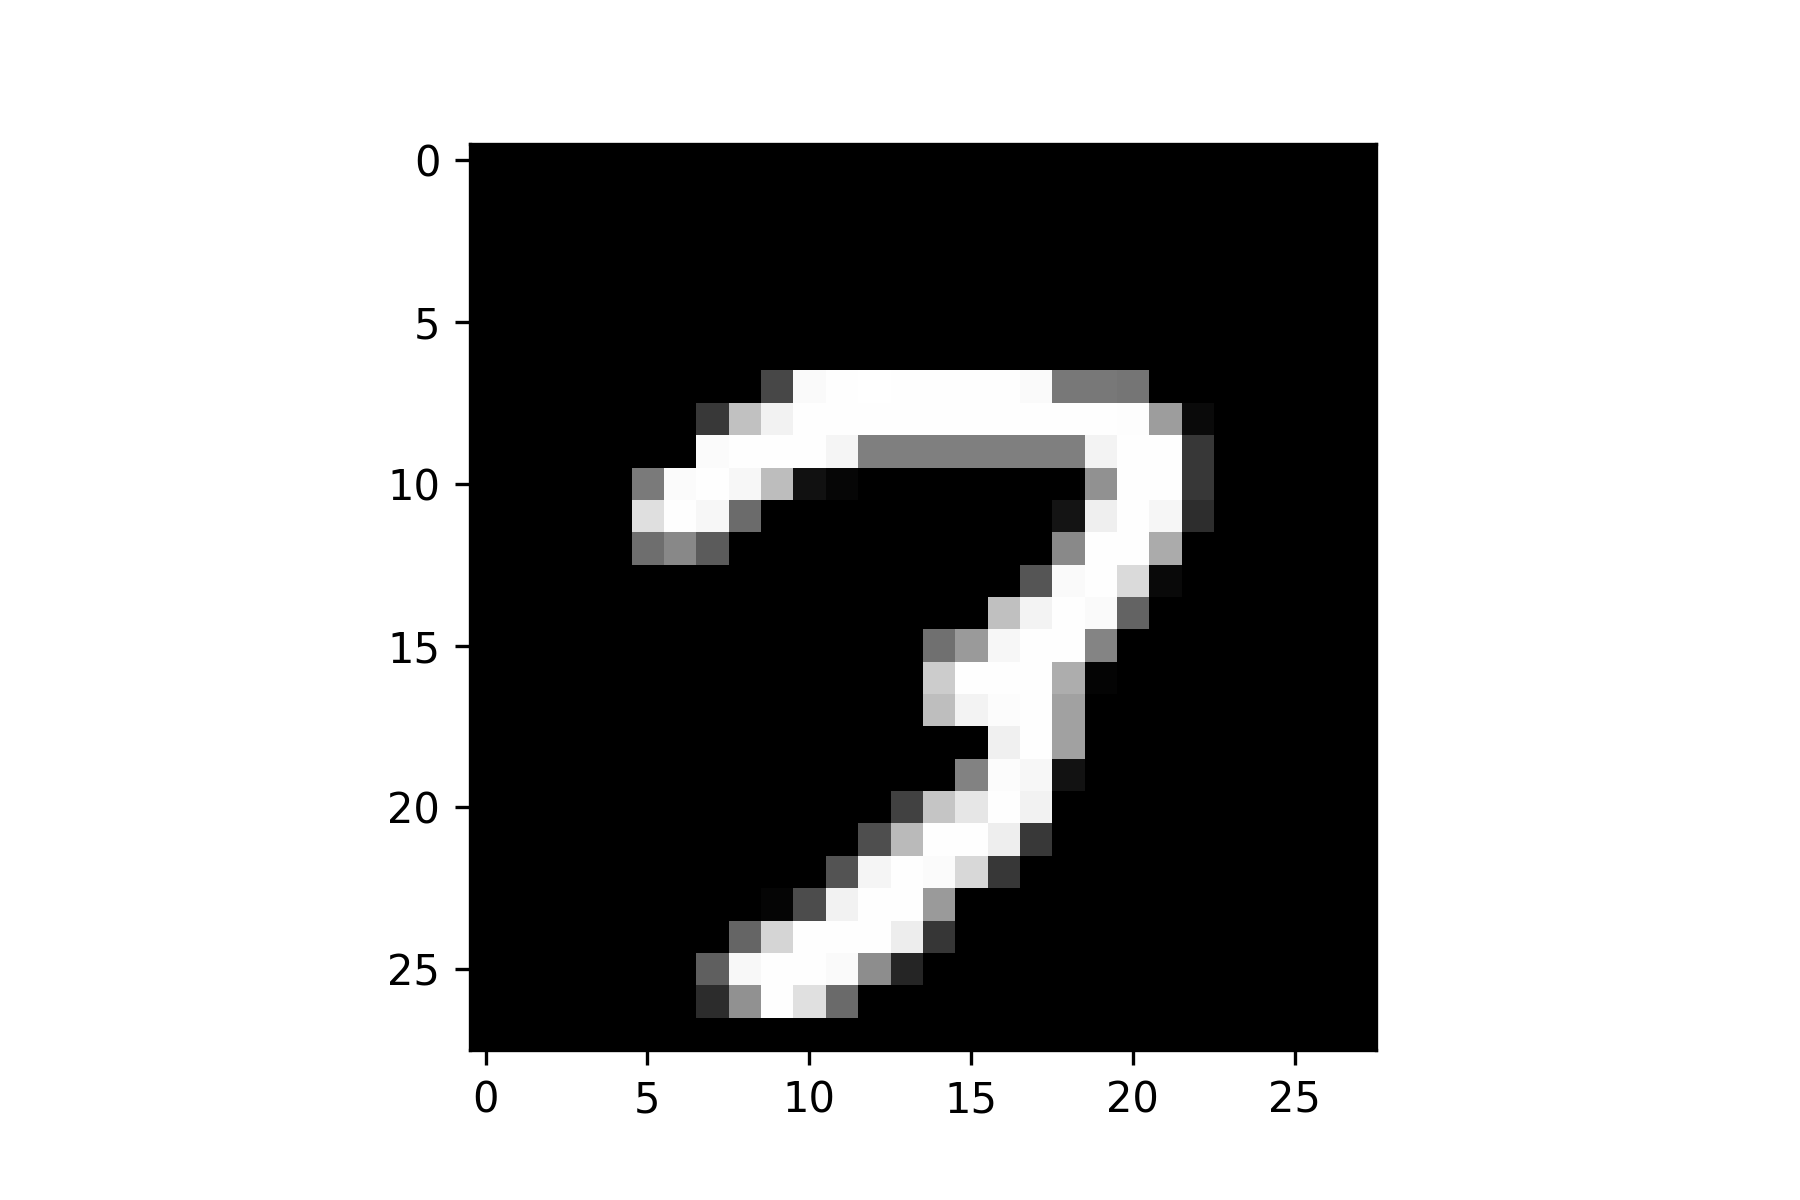
\includegraphics[width=5.0cm]{8}
        \caption{
            Real class: 3 (0.12)\\
            Predicted class: 7 (0.86)}
        \label{fig:example_1}
    \end{subfigure}
    \hfill
    % example 2
    \begin{subfigure}{0.32\textwidth}
        \centering
        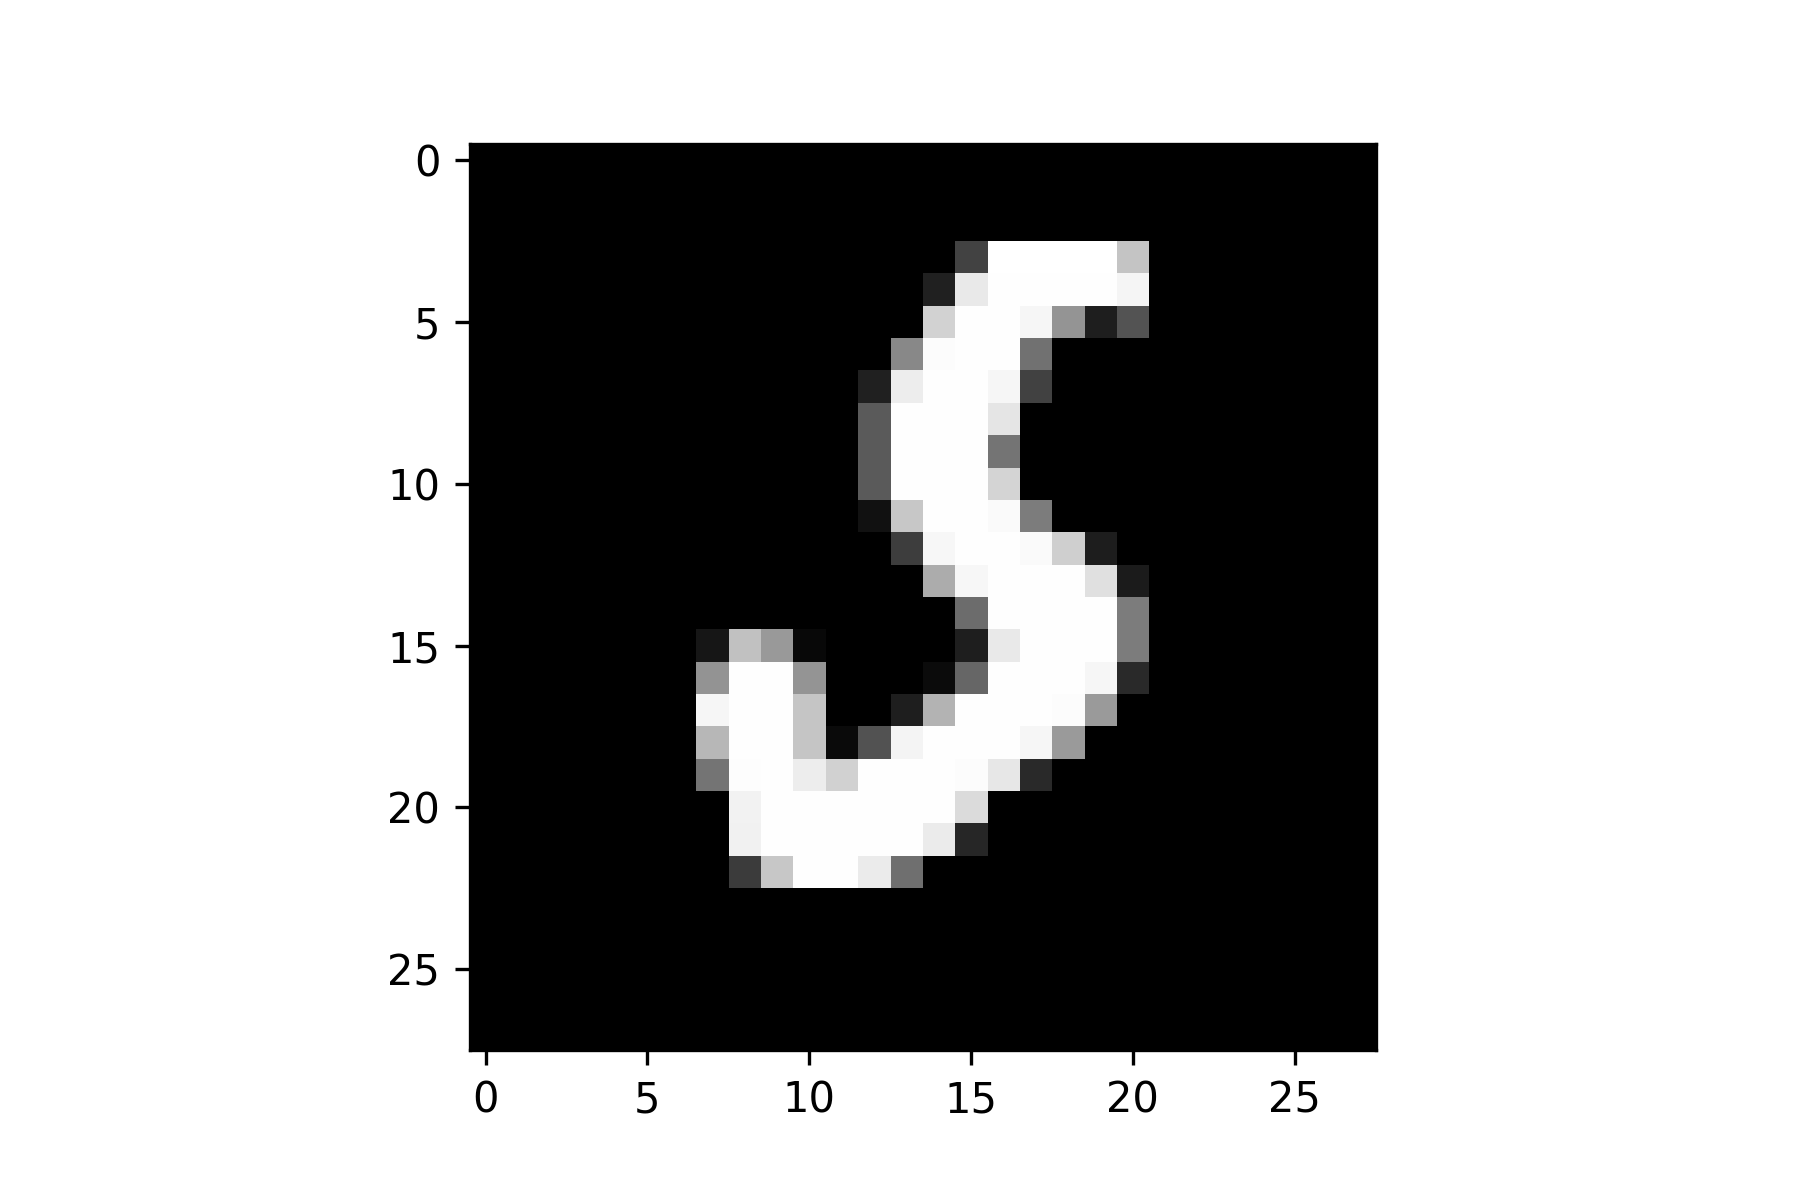
\includegraphics[width=5.0cm]{9}
        \caption{
            Real class: 5 (-0.16)\\
            Predicted class: 6 (0.57)}
        \label{fig:example_2}
    \end{subfigure}
    \hfill
    % example 3
    \begin{subfigure}{0.32\textwidth}
        \centering
        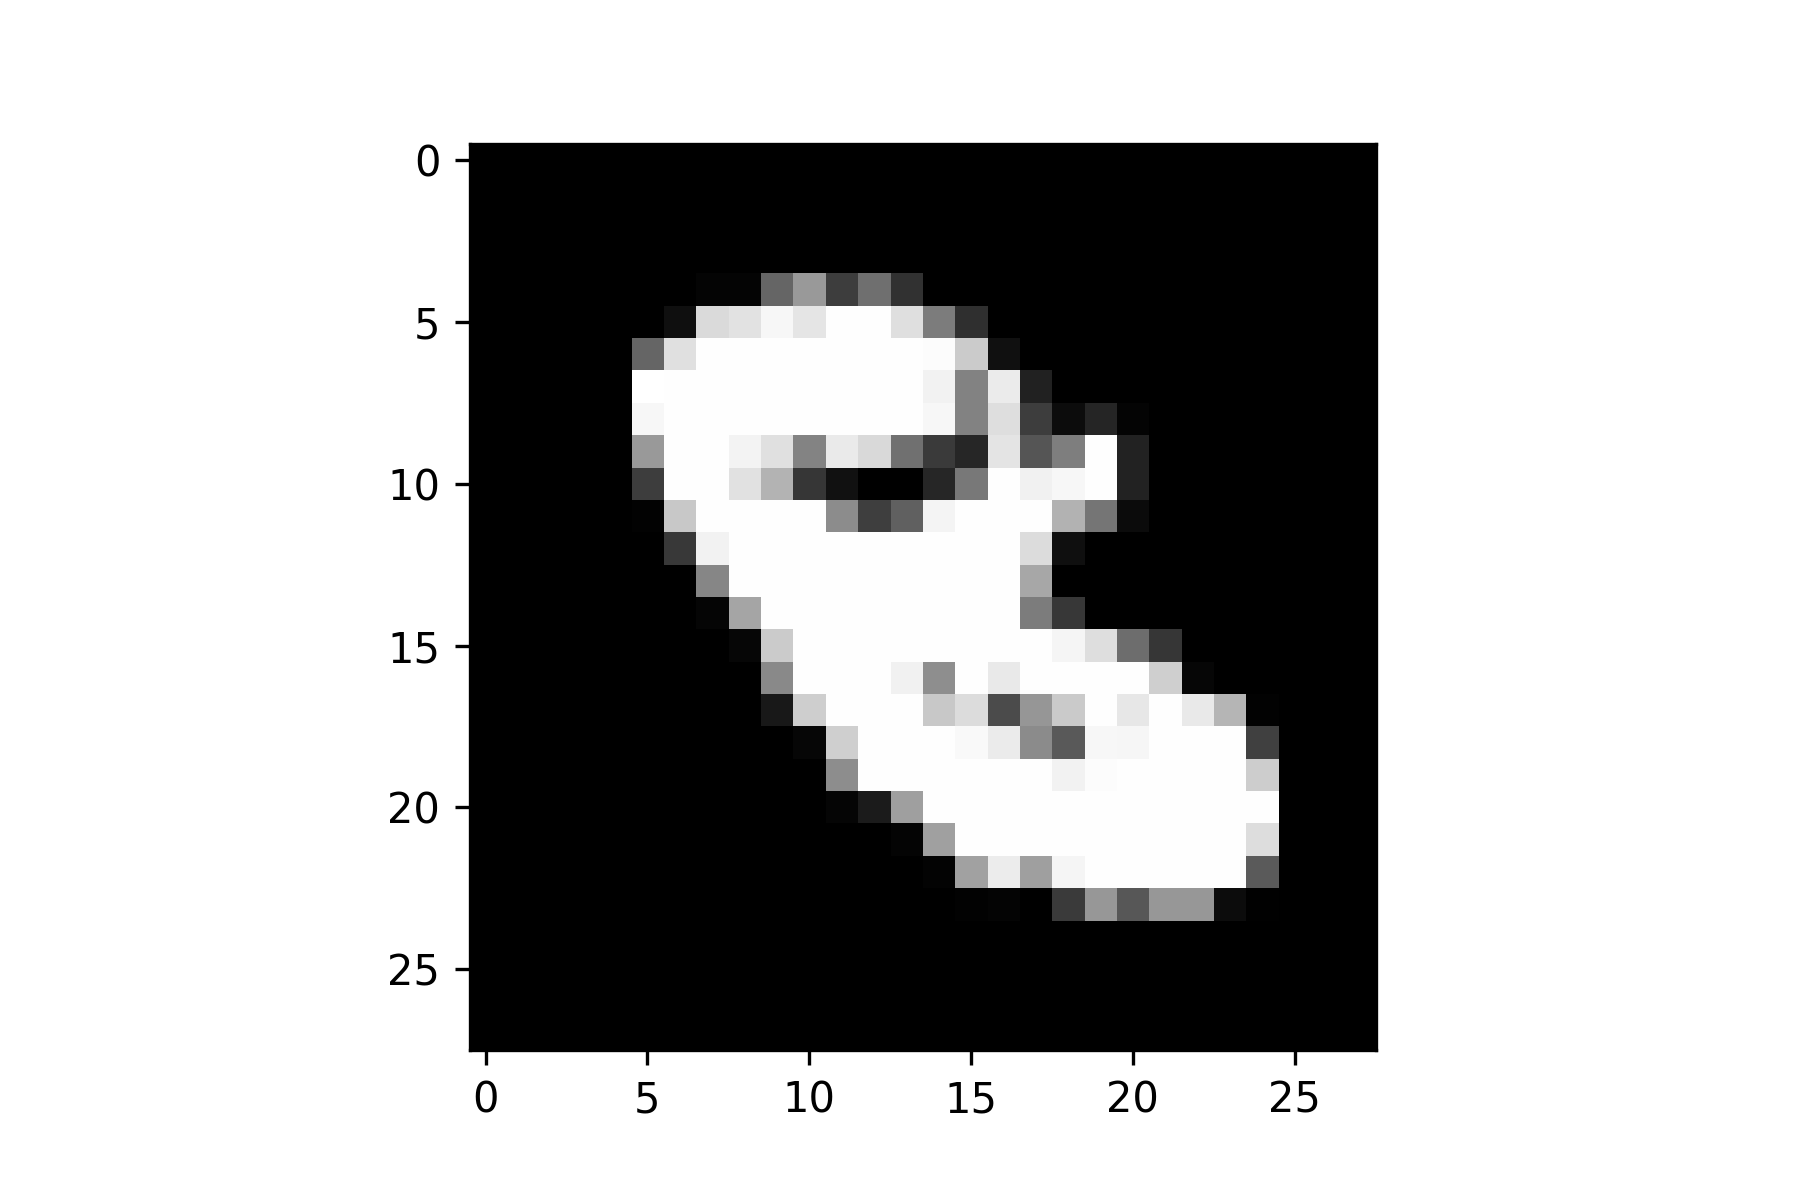
\includegraphics[width=5.0cm]{10}
        \caption{
            Real class: 8 (-0.00)\\
            Predicted class: 2 (0.72)}
        \label{fig:example_3}
    \end{subfigure}
    \hfill
    % example 4
    \begin{subfigure}{0.32\textwidth}
        \centering
        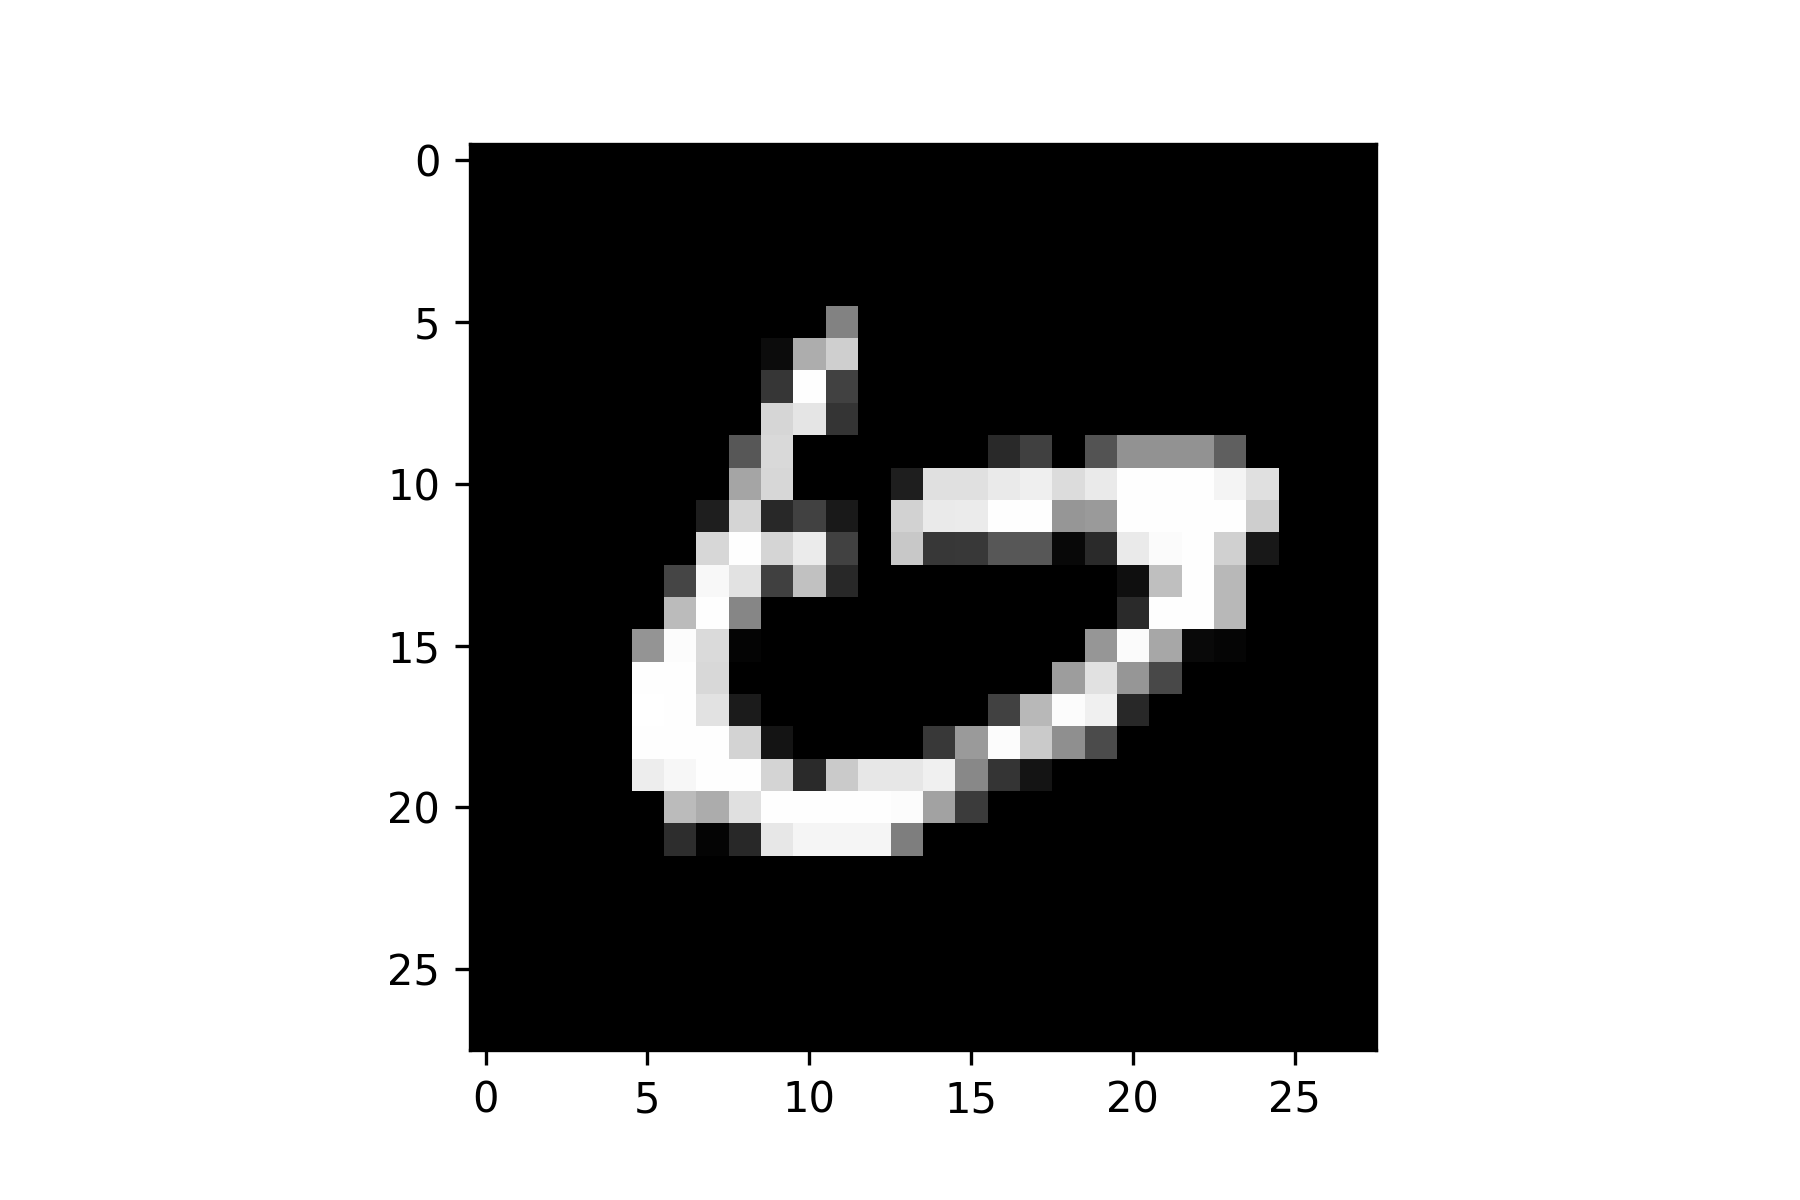
\includegraphics[width=5.0cm]{12}
        \caption{
            Real class: 6 (0.06)\\
            Predicted class: 0 (0.76)}
        \label{fig:example_4}
    \end{subfigure}
    \hfill
    % example 5
    \begin{subfigure}{0.32\textwidth}
        \centering
        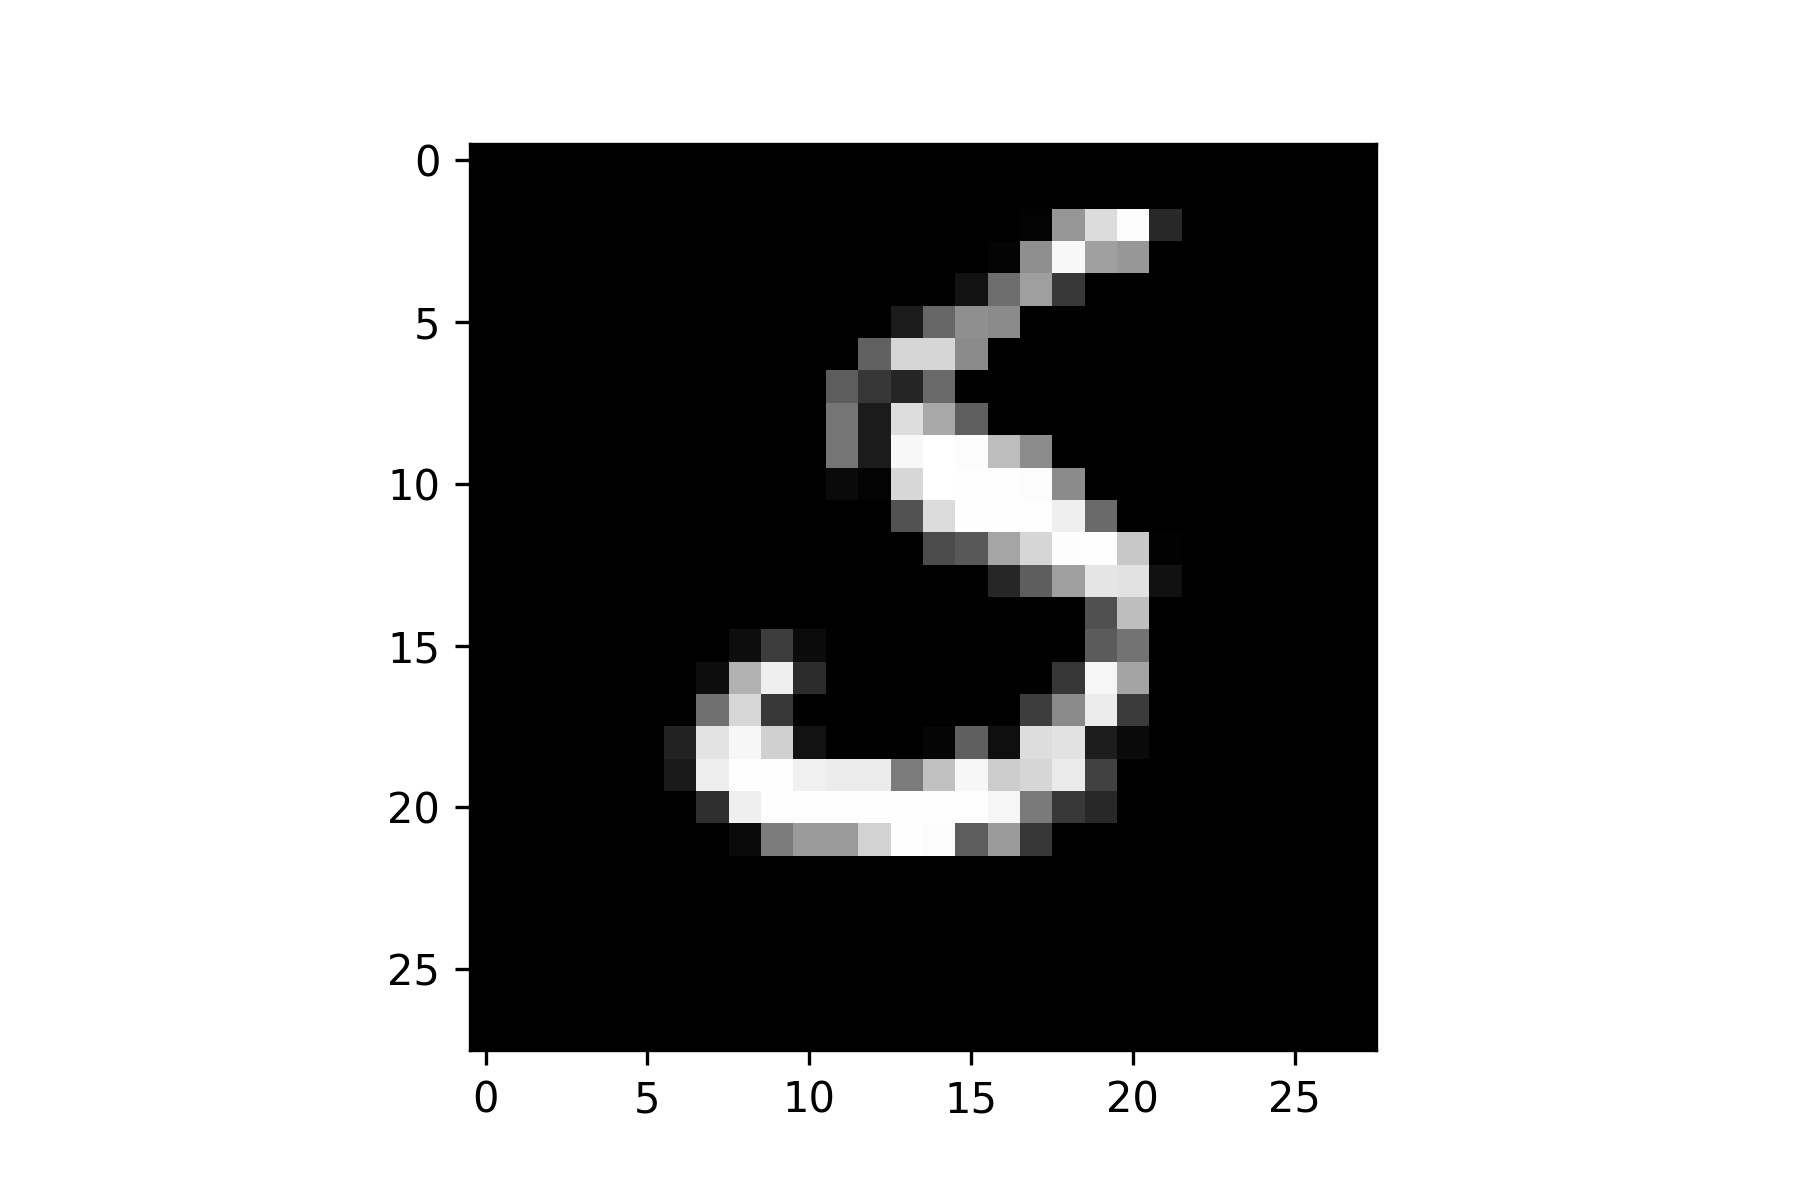
\includegraphics[width=5.0cm]{14}
        \caption{
            Real class: 5 (-0.10)\\
            Predicted class: 6 (0.58)}
        \label{fig:example_5}
    \end{subfigure}
    \hfill
    % example 6
    \begin{subfigure}{0.32\textwidth}
        \centering
        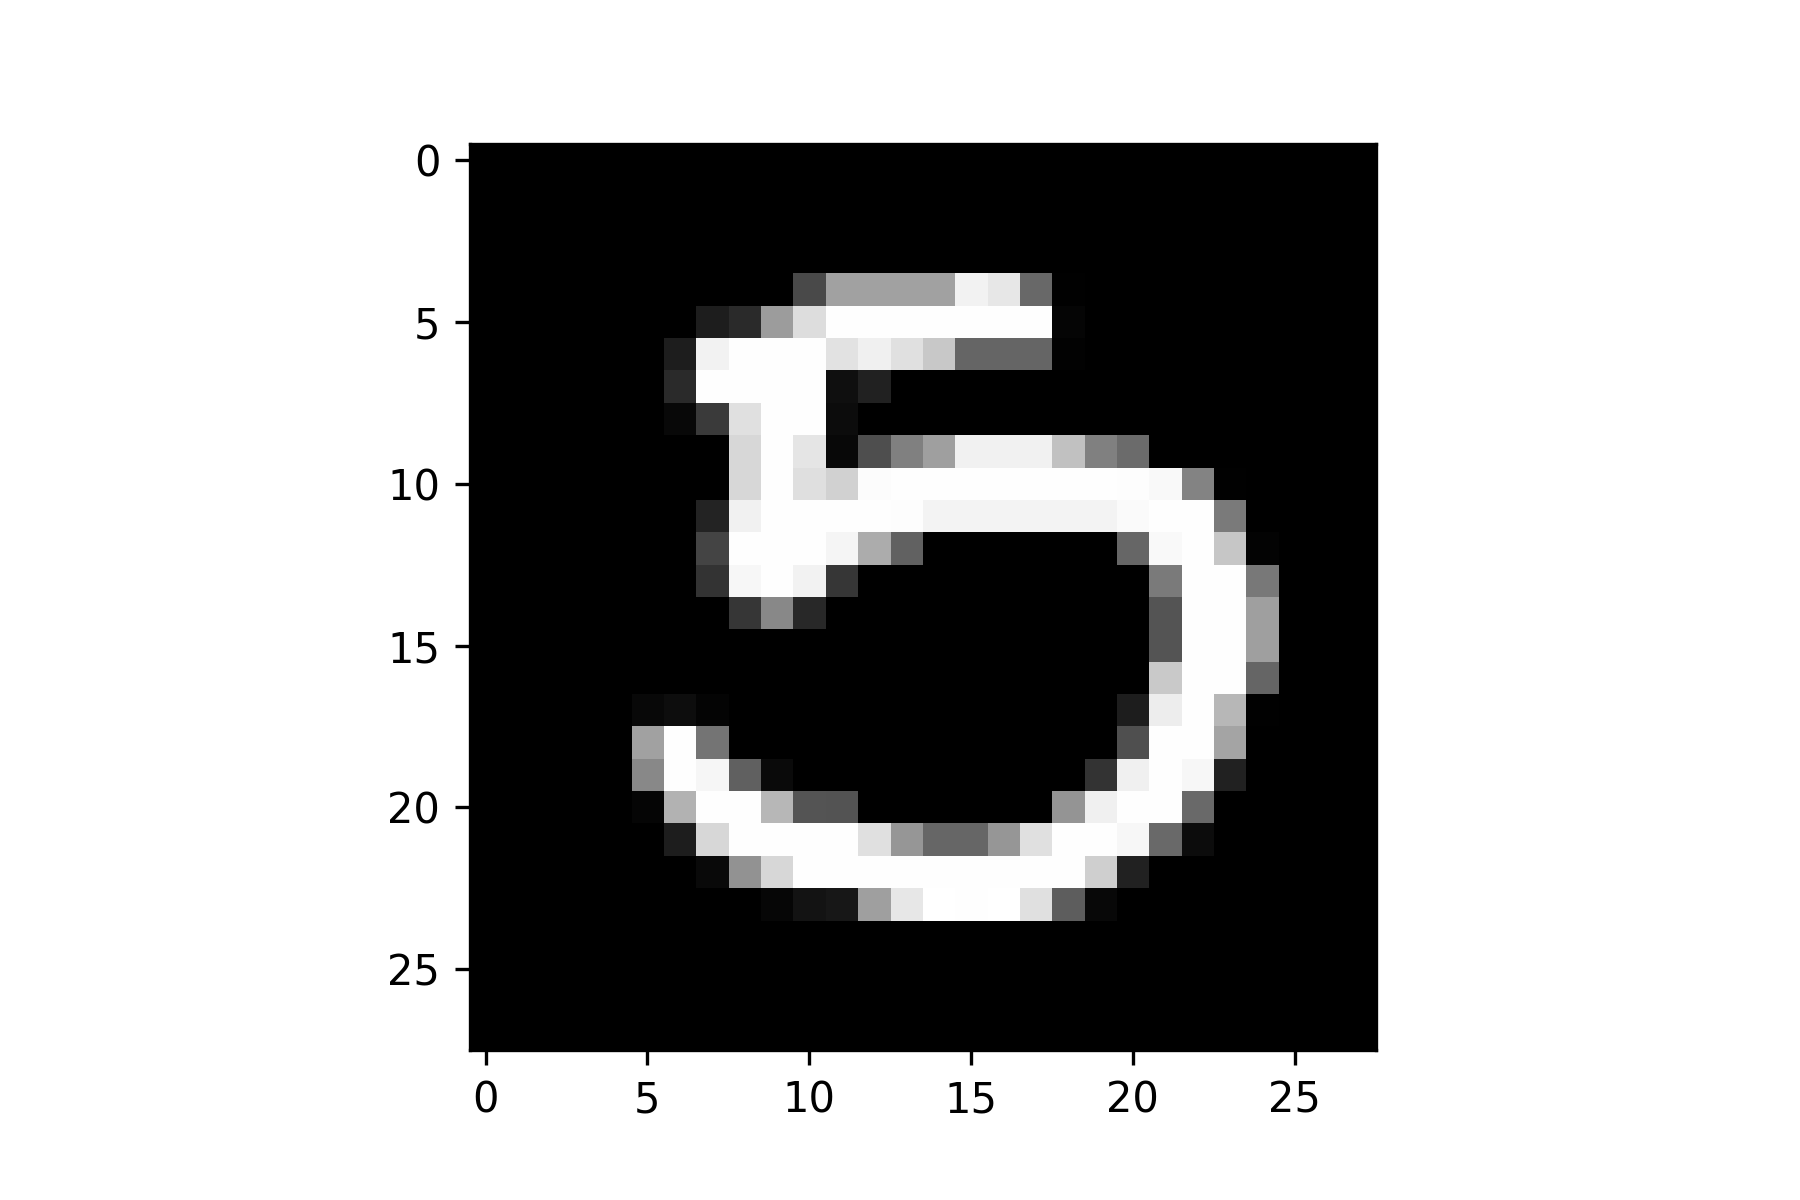
\includegraphics[width=5.0cm]{17}
        \caption{
            Real class: 5 (0.04)\\
            Predicted class: 0 (0.71)}
        \label{fig:example_6}
    \end{subfigure}
    \hfill
    % example 7
    \begin{subfigure}{0.32\textwidth}
        \centering
        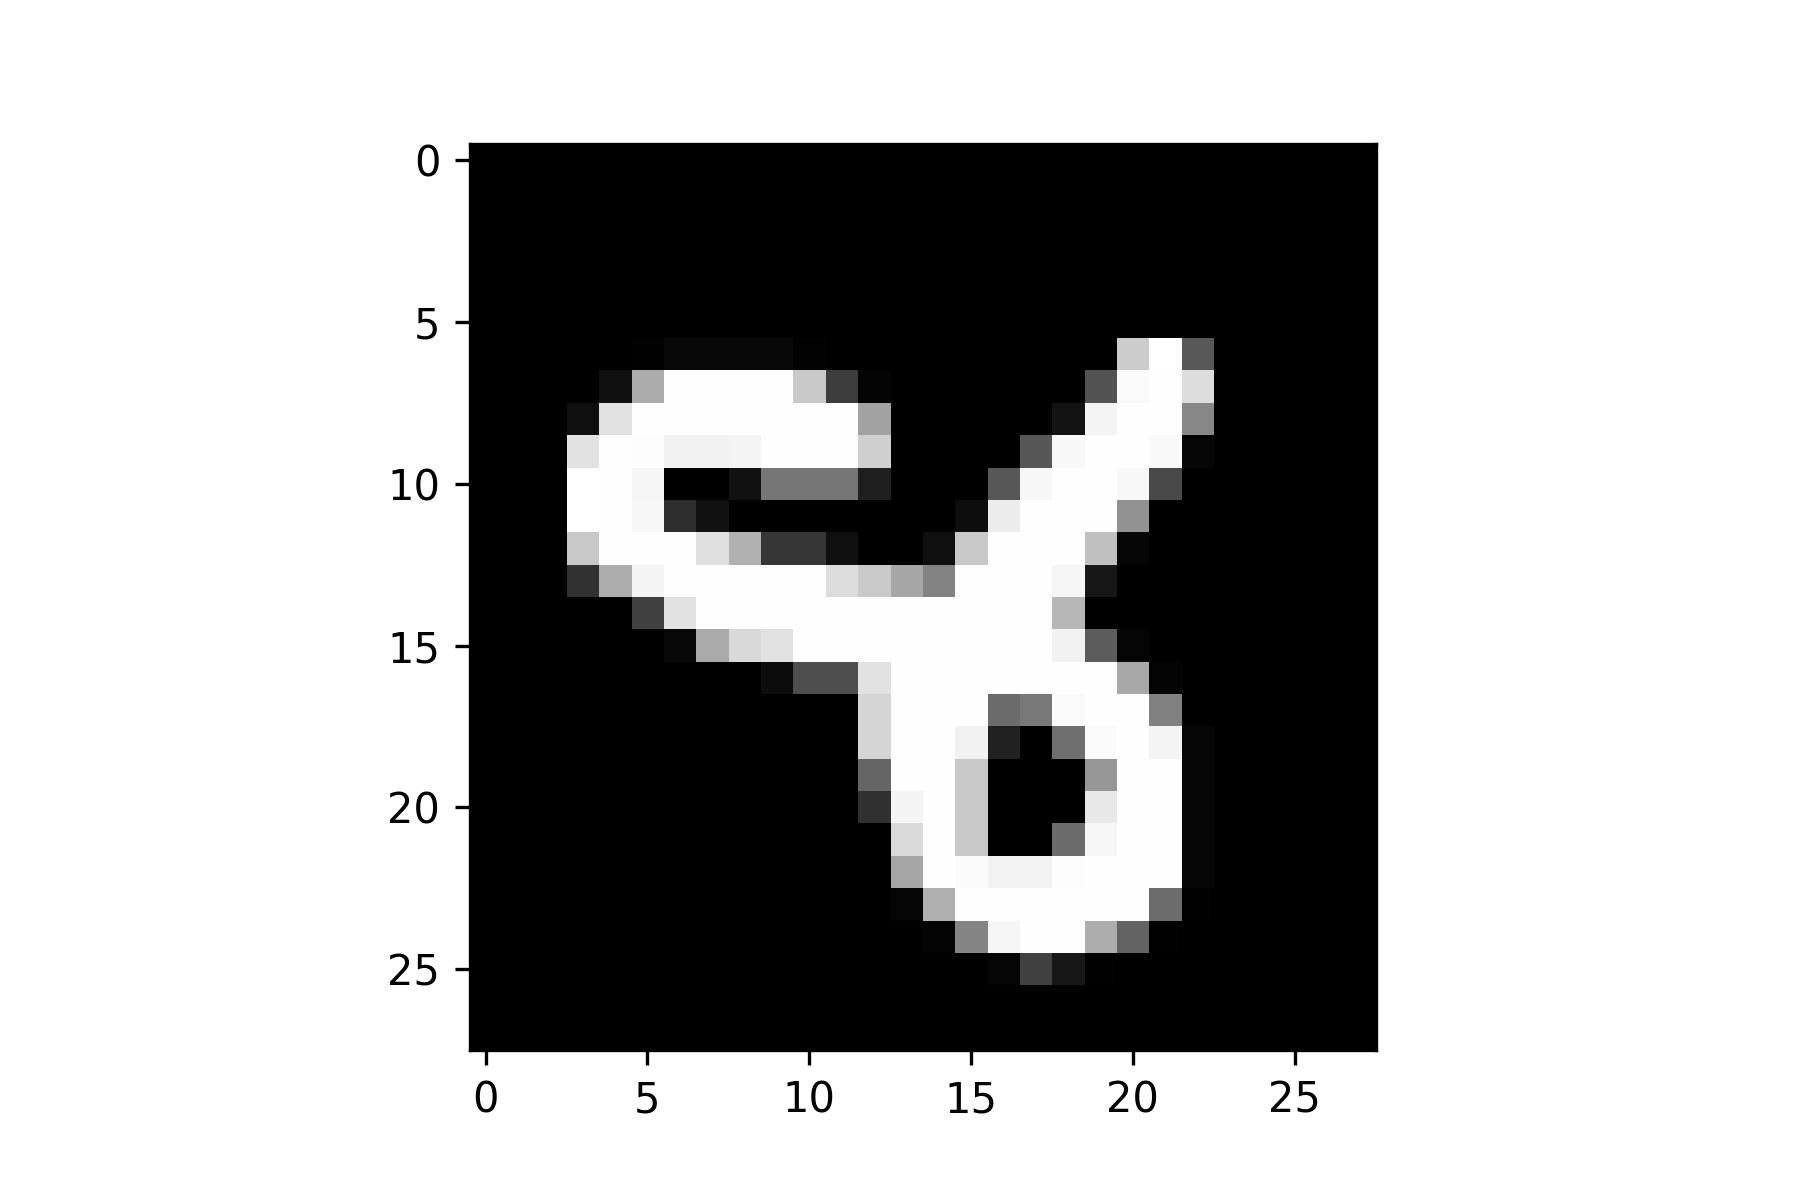
\includegraphics[width=5.0cm]{19}
        \caption{
            Real class: 8 (0.16)\\
            Predicted class: 4 (0.79)}
        \label{fig:example_7}
    \end{subfigure}
    \hfill
    % example 8
    \begin{subfigure}{0.32\textwidth}
        \centering
        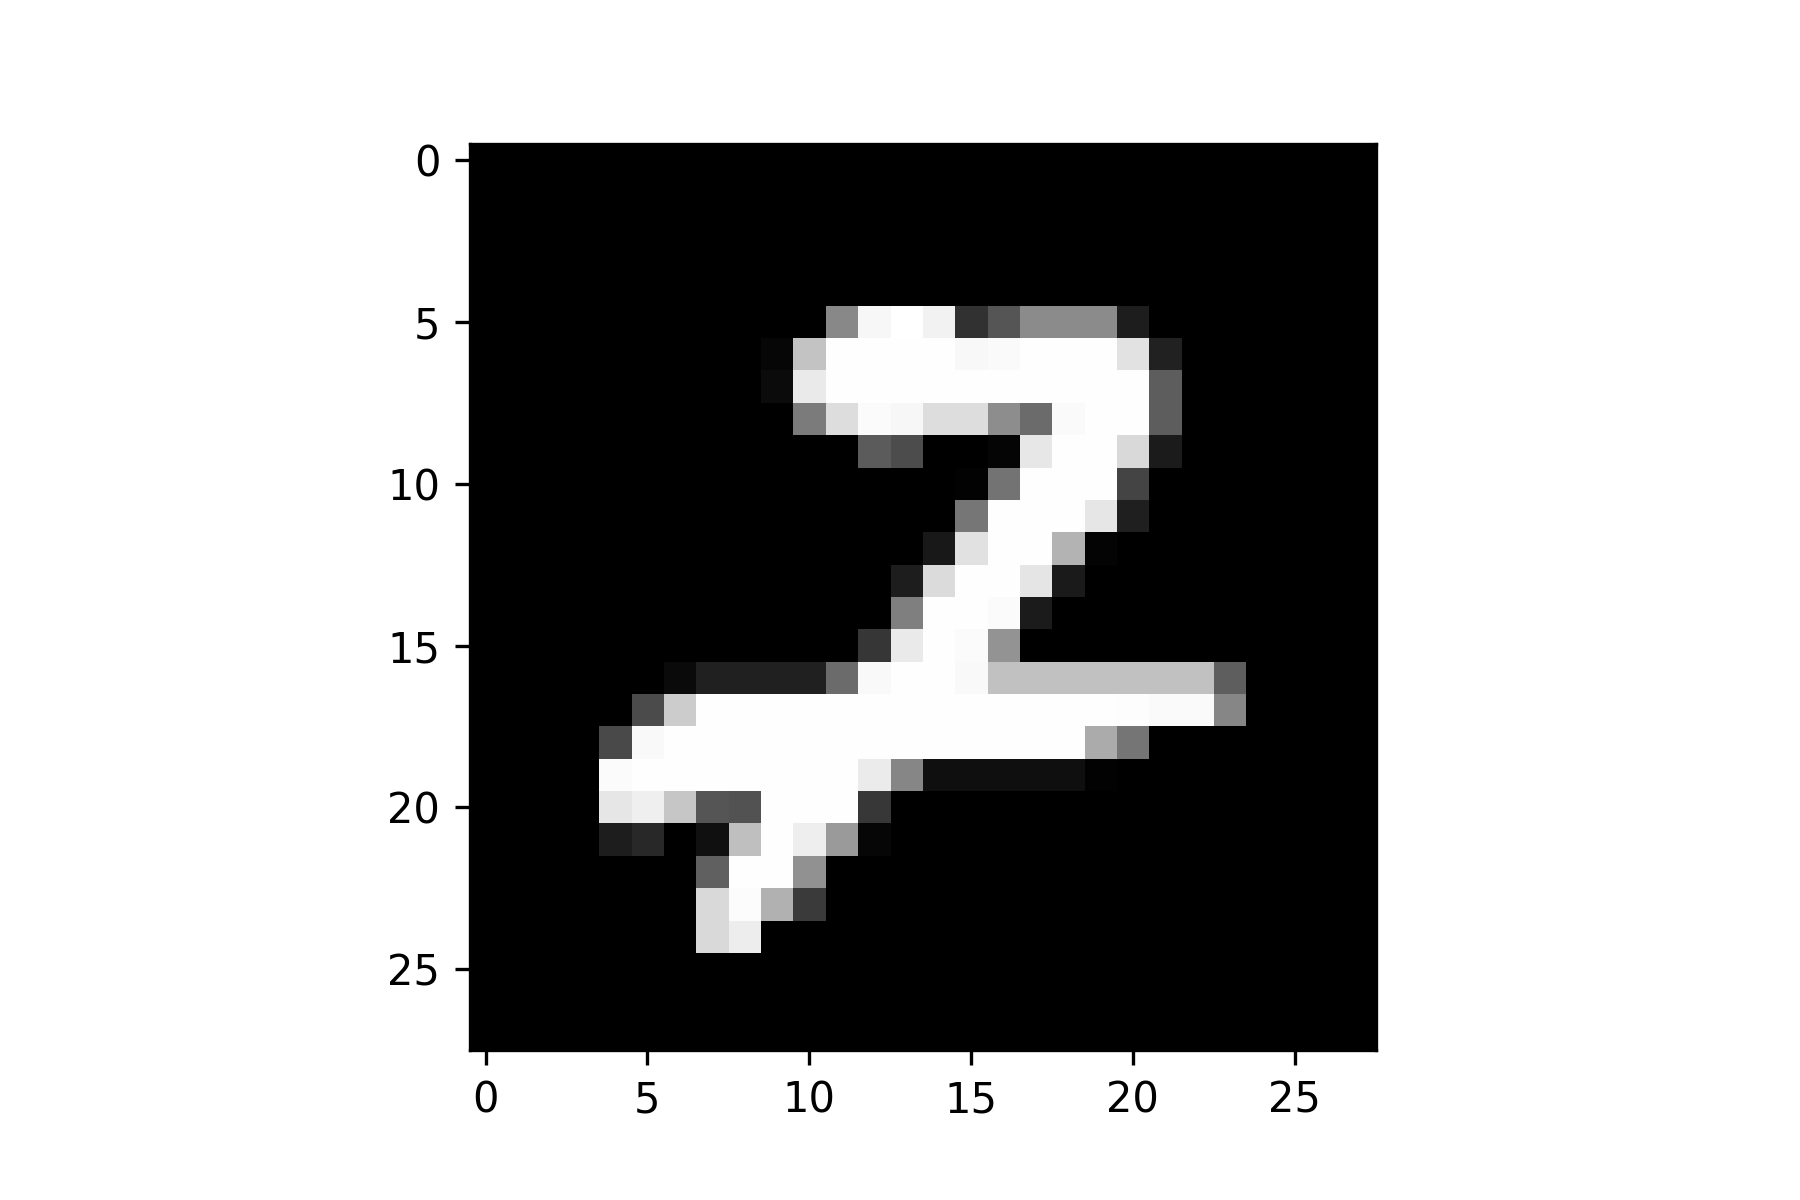
\includegraphics[width=5.0cm]{21}
        \caption{
            Real class: 7 (-0.01)\\
            Predicted class: 2 (0.63)}
        \label{fig:example_8}
    \end{subfigure}
    \hfill
    % example 9
    \begin{subfigure}{0.32\textwidth}
        \centering
        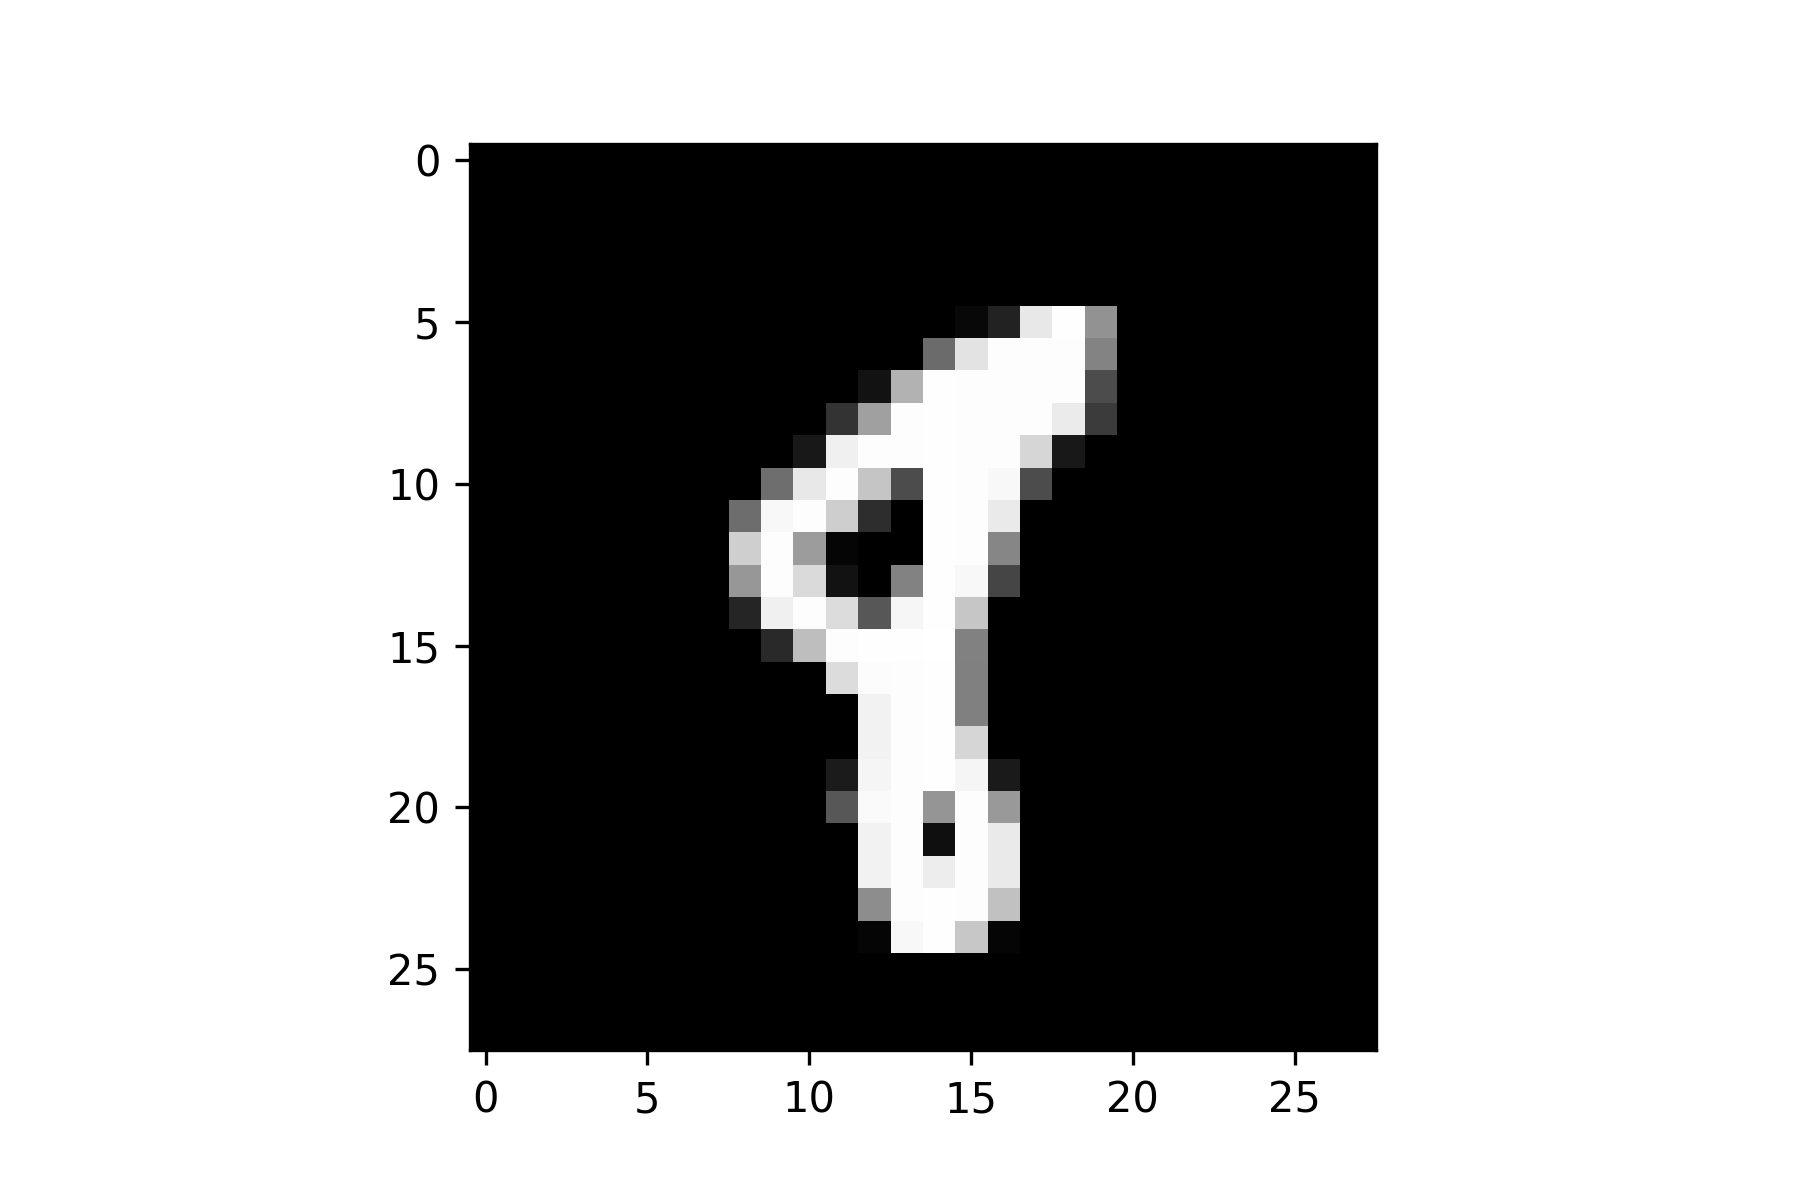
\includegraphics[width=5.0cm]{24}
        \caption{
            Real class: 8 (0.12)\\
            Predicted class: 1 (0.75)}
        \label{fig:example_9}
    \end{subfigure}
    \hfill
    % example 10
    \begin{subfigure}{0.32\textwidth}
        \centering
        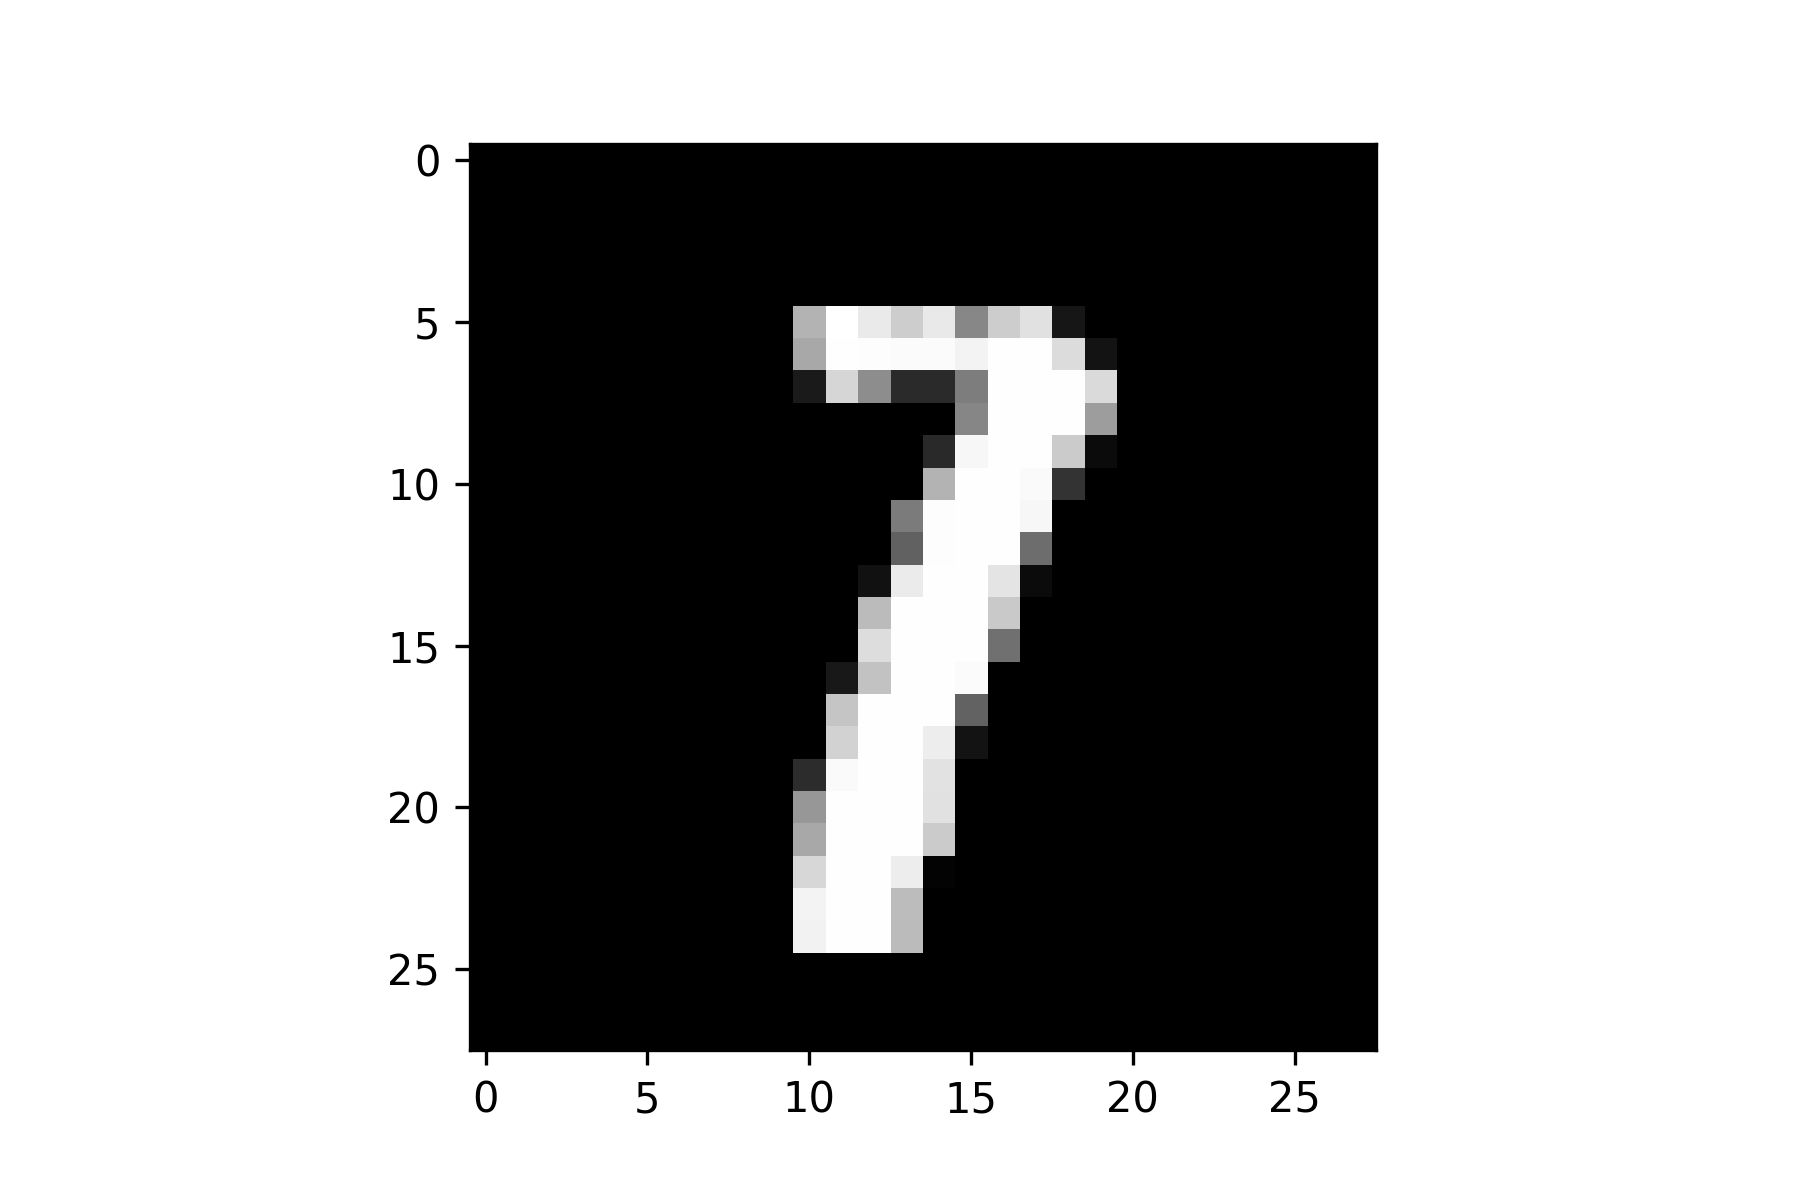
\includegraphics[width=5.0cm]{26}
        \caption{
            Real class: 1 (0.04)\\
            Predicted class: 7 (0.64)}
        \label{fig:example_10}
    \end{subfigure}
    \hfill
    % example 11
    \begin{subfigure}{0.32\textwidth}
        \centering
        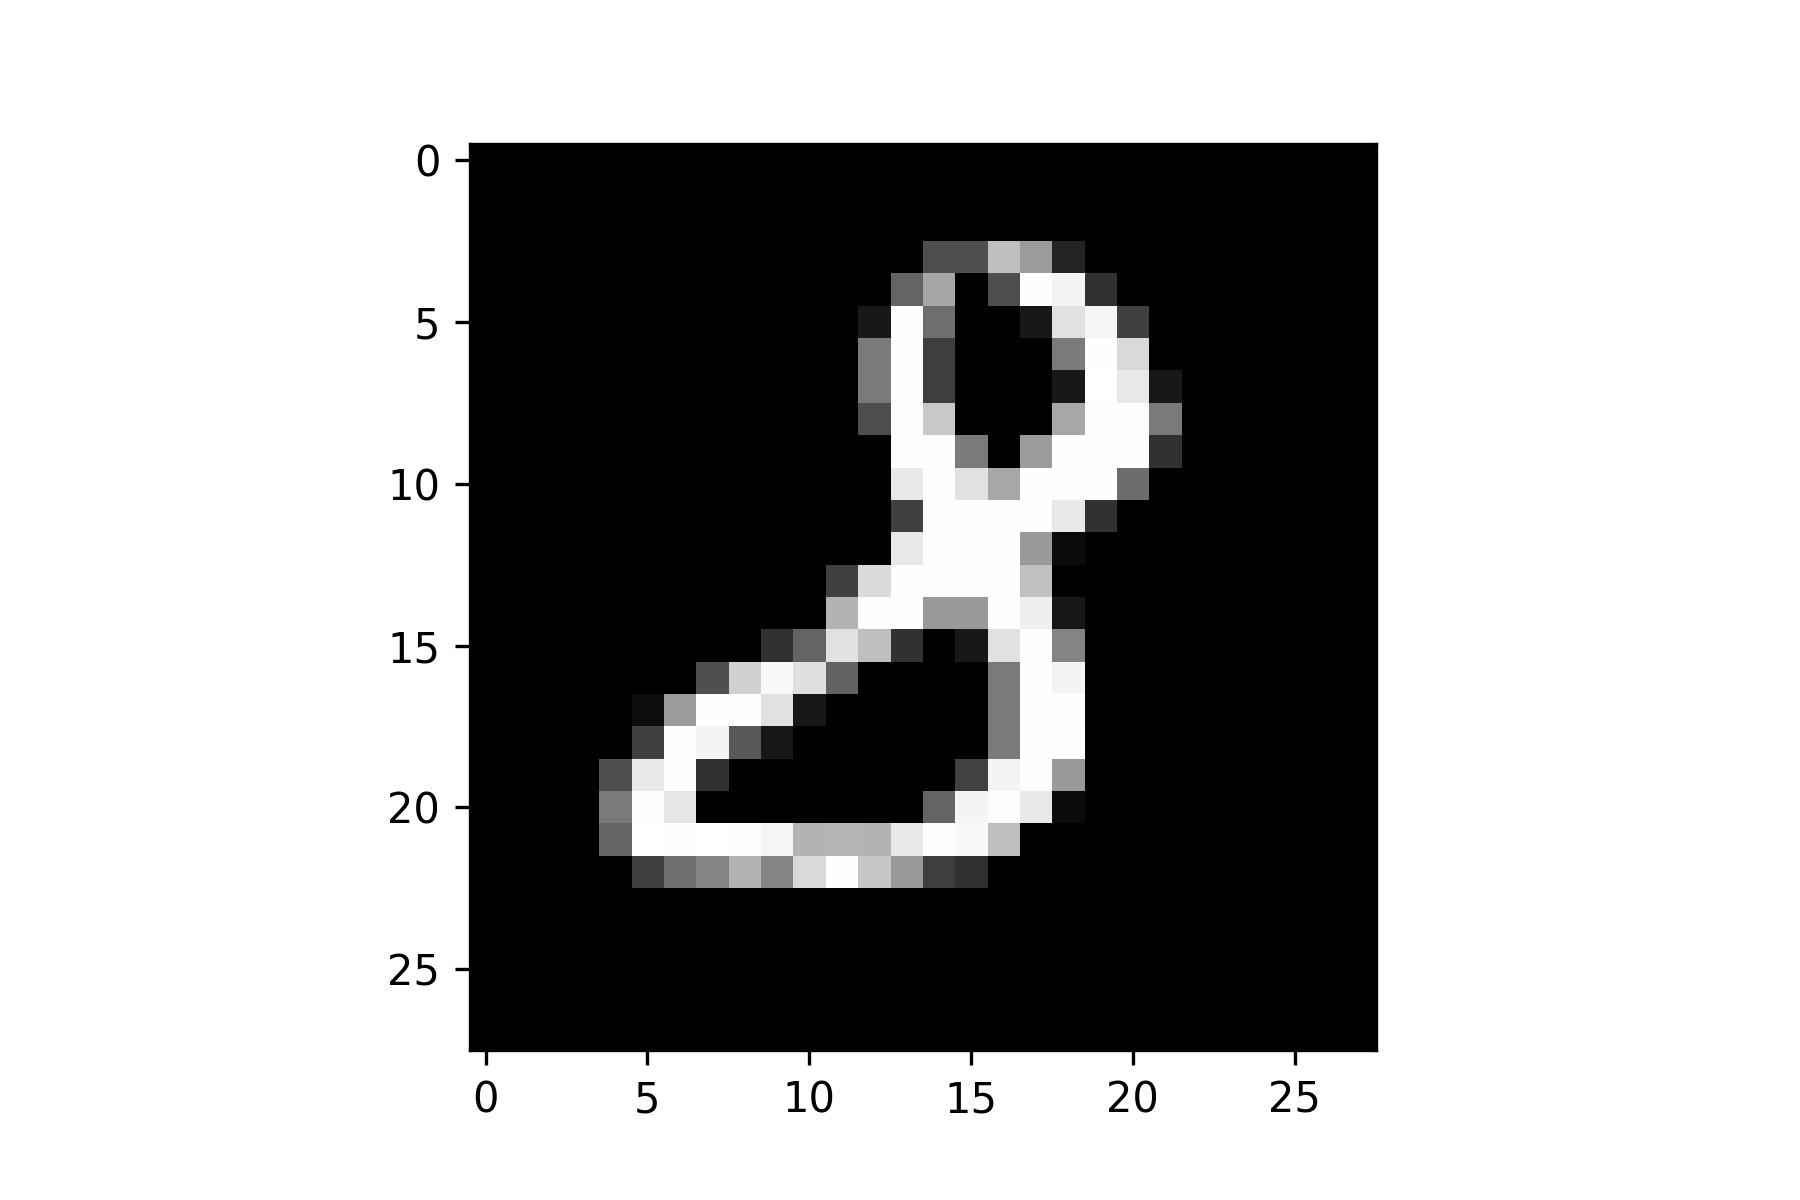
\includegraphics[width=5.0cm]{15}
        \caption{
            Real class: 8 (-0.15)\\
            Predicted class: 3 (0.53)}
        \label{fig:example_11}
    \end{subfigure}
    \hfill
     % example 12
    \begin{subfigure}{0.32\textwidth}
        \centering
        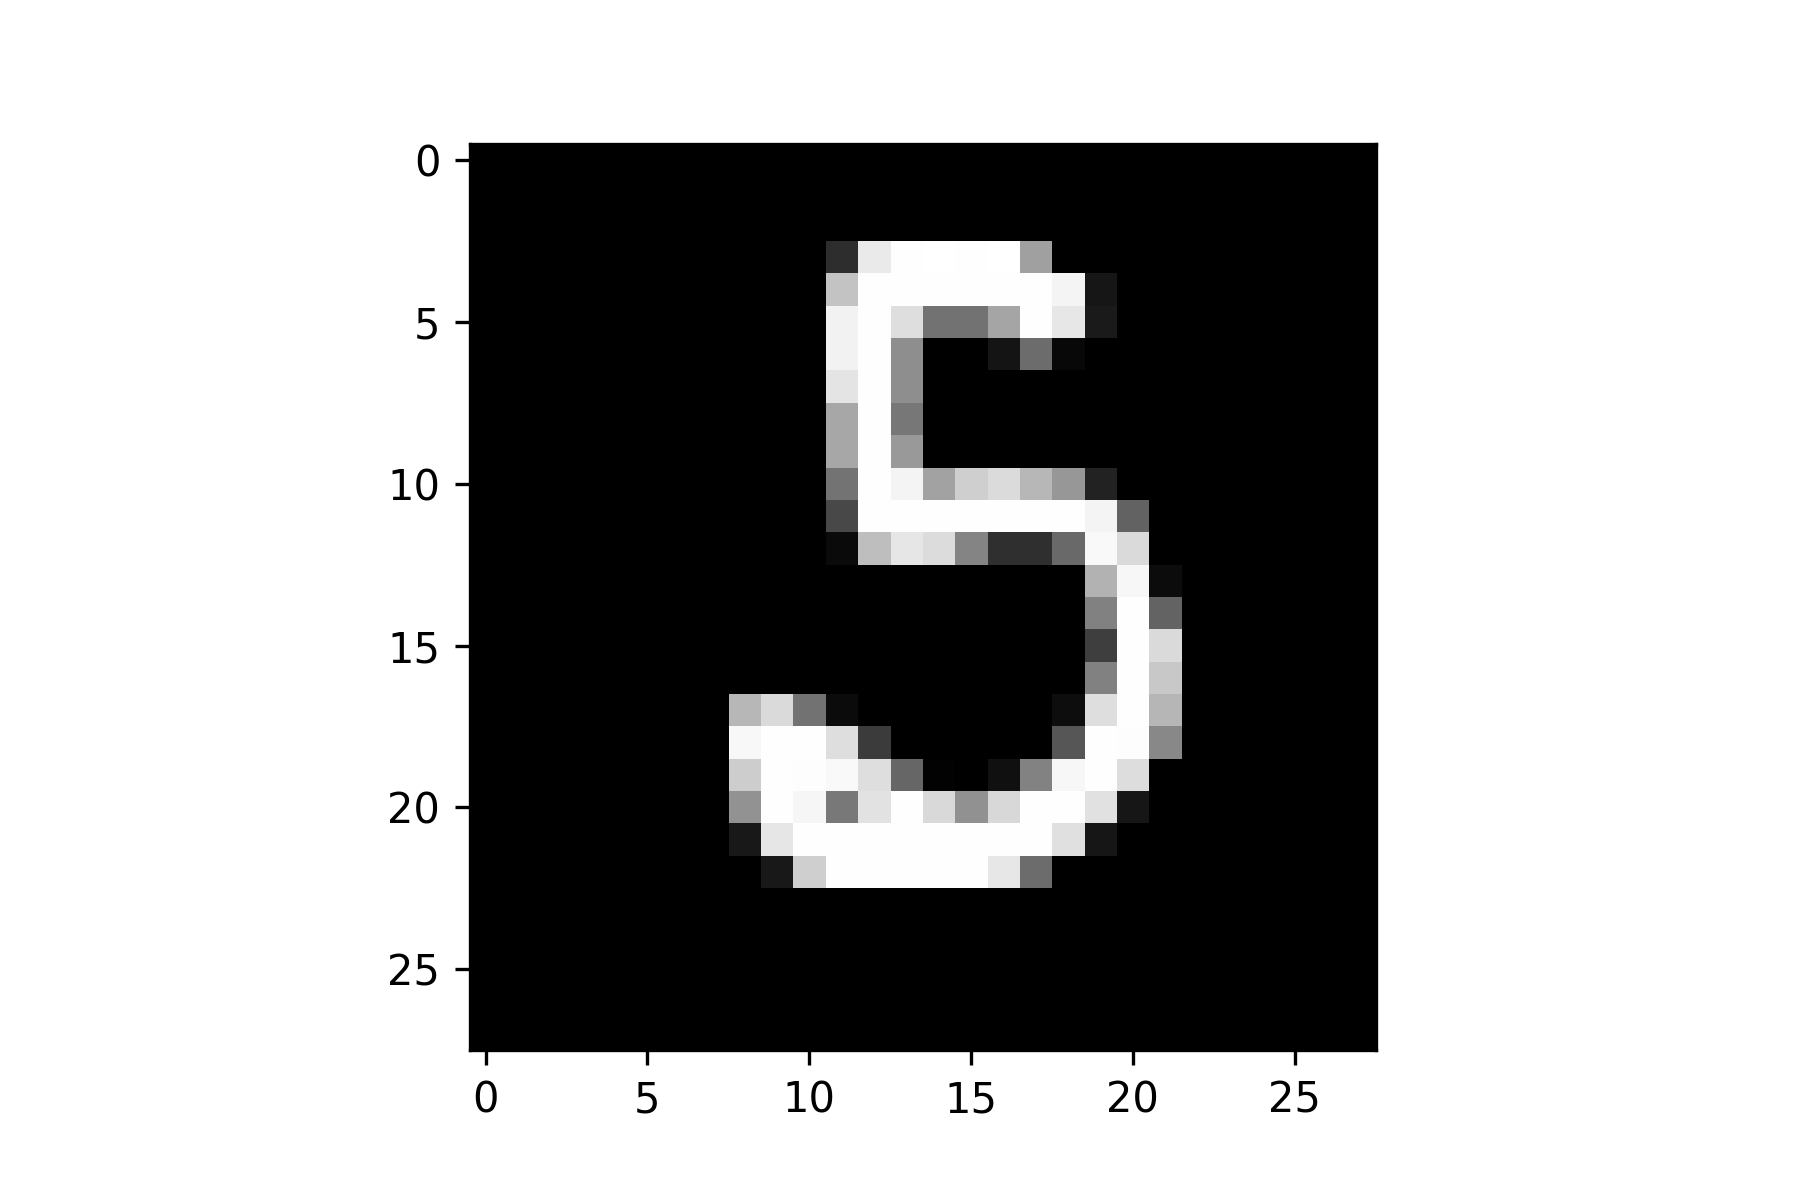
\includegraphics[width=5.0cm]{20}
        \caption{
            Real class: 5 (-0.05)\\
            Predicted class: 6 (0.58)}
        \label{fig:example_12}
    \end{subfigure}
    \hfill
    % caption and label
    \caption{Misclassified digits} 
    \label{fig:misclassified_digits}
\end{figure}

\newpage
%=================================================
\section{Theoretical question}
%=================================================

\paragraph{\textbf{Question:}\\
The choice of a different regularization coefficient for each class (instead of a single value for all classes) can give a higher performance?}

\paragraph{\textbf{Answer:}\\
...to\_be\_answered...}

%=================================================
\end{document}
